\documentclass{acm_proc_article-sp}
%\usepackage{hyperref}
\usepackage{graphicx}
\usepackage{color}
\usepackage{listings}
\usepackage{epsfig}
\usepackage[all]{xy}

%% ODER: format ==         = "\mathrel{==}"
%% ODER: format /=         = "\neq "
%
%
\makeatletter
\@ifundefined{lhs2tex.lhs2tex.sty.read}%
  {\@namedef{lhs2tex.lhs2tex.sty.read}{}%
   \newcommand\SkipToFmtEnd{}%
   \newcommand\EndFmtInput{}%
   \long\def\SkipToFmtEnd#1\EndFmtInput{}%
  }\SkipToFmtEnd

\newcommand\ReadOnlyOnce[1]{\@ifundefined{#1}{\@namedef{#1}{}}\SkipToFmtEnd}
\usepackage{amstext}
\usepackage{amssymb}
\usepackage{stmaryrd}
\DeclareFontFamily{OT1}{cmtex}{}
\DeclareFontShape{OT1}{cmtex}{m}{n}
  {<5><6><7><8>cmtex8
   <9>cmtex9
   <10><10.95><12><14.4><17.28><20.74><24.88>cmtex10}{}
\DeclareFontShape{OT1}{cmtex}{m}{it}
  {<-> ssub * cmtt/m/it}{}
\newcommand{\texfamily}{\fontfamily{cmtex}\selectfont}
\DeclareFontShape{OT1}{cmtt}{bx}{n}
  {<5><6><7><8>cmtt8
   <9>cmbtt9
   <10><10.95><12><14.4><17.28><20.74><24.88>cmbtt10}{}
\DeclareFontShape{OT1}{cmtex}{bx}{n}
  {<-> ssub * cmtt/bx/n}{}
\newcommand{\tex}[1]{\text{\texfamily#1}}	% NEU

\newcommand{\Sp}{\hskip.33334em\relax}


\newcommand{\Conid}[1]{\mathit{#1}}
\newcommand{\Varid}[1]{\mathit{#1}}
\newcommand{\anonymous}{\kern0.06em \vbox{\hrule\@width.5em}}
\newcommand{\plus}{\mathbin{+\!\!\!+}}
\newcommand{\bind}{\mathbin{>\!\!\!>\mkern-6.7mu=}}
\newcommand{\rbind}{\mathbin{=\mkern-6.7mu<\!\!\!<}}% suggested by Neil Mitchell
\newcommand{\sequ}{\mathbin{>\!\!\!>}}
\renewcommand{\leq}{\leqslant}
\renewcommand{\geq}{\geqslant}
\usepackage{polytable}

%mathindent has to be defined
\@ifundefined{mathindent}%
  {\newdimen\mathindent\mathindent\leftmargini}%
  {}%

\def\resethooks{%
  \global\let\SaveRestoreHook\empty
  \global\let\ColumnHook\empty}
\newcommand*{\savecolumns}[1][default]%
  {\g@addto@macro\SaveRestoreHook{\savecolumns[#1]}}
\newcommand*{\restorecolumns}[1][default]%
  {\g@addto@macro\SaveRestoreHook{\restorecolumns[#1]}}
\newcommand*{\aligncolumn}[2]%
  {\g@addto@macro\ColumnHook{\column{#1}{#2}}}

\resethooks

\newcommand{\onelinecommentchars}{\quad-{}- }
\newcommand{\commentbeginchars}{\enskip\{-}
\newcommand{\commentendchars}{-\}\enskip}

\newcommand{\visiblecomments}{%
  \let\onelinecomment=\onelinecommentchars
  \let\commentbegin=\commentbeginchars
  \let\commentend=\commentendchars}

\newcommand{\invisiblecomments}{%
  \let\onelinecomment=\empty
  \let\commentbegin=\empty
  \let\commentend=\empty}

\visiblecomments

\newlength{\blanklineskip}
\setlength{\blanklineskip}{1mm}

\newcommand{\hsindent}[1]{\quad}% default is fixed indentation
\let\hspre\empty
\let\hspost\empty
\newcommand{\NB}{\textbf{NB}}
\newcommand{\Todo}[1]{$\langle$\textbf{To do:}~#1$\rangle$}

\EndFmtInput
\makeatother
%
%
%
%
%
%
% This package provides two environments suitable to take the place
% of hscode, called "plainhscode" and "arrayhscode". 
%
% The plain environment surrounds each code block by vertical space,
% and it uses \abovedisplayskip and \belowdisplayskip to get spacing
% similar to formulas. Note that if these dimensions are changed,
% the spacing around displayed math formulas changes as well.
% All code is indented using \leftskip.
%
% Changed 19.08.2004 to reflect changes in colorcode. Should work with
% CodeGroup.sty.
%
\ReadOnlyOnce{polycode.fmt}%
\makeatletter

\newcommand{\hsnewpar}[1]%
  {{\parskip=0pt\parindent=0pt\par\vskip #1\noindent}}

% can be used, for instance, to redefine the code size, by setting the
% command to \small or something alike
\newcommand{\hscodestyle}{}

% The command \sethscode can be used to switch the code formatting
% behaviour by mapping the hscode environment in the subst directive
% to a new LaTeX environment.

\newcommand{\sethscode}[1]%
  {\expandafter\let\expandafter\hscode\csname #1\endcsname
   \expandafter\let\expandafter\endhscode\csname end#1\endcsname}

% "compatibility" mode restores the non-polycode.fmt layout.

\newenvironment{compathscode}%
  {\par\noindent
   \advance\leftskip\mathindent
   \hscodestyle
   \let\\=\@normalcr
   \(\pboxed}%
  {\endpboxed\)%
   \par\noindent
   \ignorespacesafterend}

\newcommand{\compaths}{\sethscode{compathscode}}

% "plain" mode is the proposed default.
% It should now work with \centering.
% This required some changes. The old version
% is still available for reference as oldplainhscode.

\newenvironment{plainhscode}%
  {\hsnewpar\abovedisplayskip
   \advance\leftskip\mathindent
   \hscodestyle
   \let\hspre\(\let\hspost\)%
   \pboxed}%
  {\endpboxed%
   \hsnewpar\belowdisplayskip
   \ignorespacesafterend}

\newenvironment{oldplainhscode}%
  {\hsnewpar\abovedisplayskip
   \advance\leftskip\mathindent
   \hscodestyle
   \let\\=\@normalcr
   \(\pboxed}%
  {\endpboxed\)%
   \hsnewpar\belowdisplayskip
   \ignorespacesafterend}

% Here, we make plainhscode the default environment.

\newcommand{\plainhs}{\sethscode{plainhscode}}
\newcommand{\oldplainhs}{\sethscode{oldplainhscode}}
\plainhs

% The arrayhscode is like plain, but makes use of polytable's
% parray environment which disallows page breaks in code blocks.

\newenvironment{arrayhscode}%
  {\hsnewpar\abovedisplayskip
   \advance\leftskip\mathindent
   \hscodestyle
   \let\\=\@normalcr
   \(\parray}%
  {\endparray\)%
   \hsnewpar\belowdisplayskip
   \ignorespacesafterend}

\newcommand{\arrayhs}{\sethscode{arrayhscode}}

% The mathhscode environment also makes use of polytable's parray 
% environment. It is supposed to be used only inside math mode 
% (I used it to typeset the type rules in my thesis).

\newenvironment{mathhscode}%
  {\parray}{\endparray}

\newcommand{\mathhs}{\sethscode{mathhscode}}

% texths is similar to mathhs, but works in text mode.

\newenvironment{texthscode}%
  {\(\parray}{\endparray\)}

\newcommand{\texths}{\sethscode{texthscode}}

% The framed environment places code in a framed box.

\def\codeframewidth{\arrayrulewidth}
\RequirePackage{calc}

\newenvironment{framedhscode}%
  {\parskip=\abovedisplayskip\par\noindent
   \hscodestyle
   \arrayrulewidth=\codeframewidth
   \tabular{@{}|p{\linewidth-2\arraycolsep-2\arrayrulewidth-2pt}|@{}}%
   \hline\framedhslinecorrect\\{-1.5ex}%
   \let\endoflinesave=\\
   \let\\=\@normalcr
   \(\pboxed}%
  {\endpboxed\)%
   \framedhslinecorrect\endoflinesave{.5ex}\hline
   \endtabular
   \parskip=\belowdisplayskip\par\noindent
   \ignorespacesafterend}

\newcommand{\framedhslinecorrect}[2]%
  {#1[#2]}

\newcommand{\framedhs}{\sethscode{framedhscode}}

% The inlinehscode environment is an experimental environment
% that can be used to typeset displayed code inline.

\newenvironment{inlinehscode}%
  {\(\def\column##1##2{}%
   \let\>\undefined\let\<\undefined\let\\\undefined
   \newcommand\>[1][]{}\newcommand\<[1][]{}\newcommand\\[1][]{}%
   \def\fromto##1##2##3{##3}%
   \def\nextline{}}{\) }%

\newcommand{\inlinehs}{\sethscode{inlinehscode}}

% The joincode environment is a separate environment that
% can be used to surround and thereby connect multiple code
% blocks.

\newenvironment{joincode}%
  {\let\orighscode=\hscode
   \let\origendhscode=\endhscode
   \def\endhscode{\def\hscode{\endgroup\def\@currenvir{hscode}\\}\begingroup}
   %\let\SaveRestoreHook=\empty
   %\let\ColumnHook=\empty
   %\let\resethooks=\empty
   \orighscode\def\hscode{\endgroup\def\@currenvir{hscode}}}%
  {\origendhscode
   \global\let\hscode=\orighscode
   \global\let\endhscode=\origendhscode}%

\makeatother
\EndFmtInput
%





\begin{document}
\lstset{language=Haskell, numbers=left,
numberstyle=\tiny,numbersep=5pt,basicstyle=\scriptsize,aboveskip=20pt}

\title{Scenario Variability as Crosscutting}


\numberofauthors{2}

\author{
\alignauthor
Rodrigo Bonif\'{a}cio\\
       \affaddr{Informatics Center}\\
       \affaddr{Federal University of Pernambuco}\\
       \affaddr{Recife, Brazil}\\
       \email{rba2@cin.ufpe.br}
\alignauthor
Paulo Borba\\
       \affaddr{Informatics Center}\\
       \affaddr{Federal University of Pernambuco}\\
       \affaddr{Recife, Brazil}\\
       \email{phmb@cin.ufpe.br}
}

\maketitle

\begin{abstract}
Variability management is a common challenge for Software Product
Line (SPL) adoption, since developers need suitable
mechanisms for specifying and implementing variability
that occurs at different SPL artifacts (requirements, design,
implementation, and test). In this paper, we present a novel approach for
use case scenario variability management, enabling a better
separation of concerns between languages used to manage
variabilities and languages used to specify use case scenarios. The
result is that both representations can be understood and evolved in
a separate way. We achieve such a goal by modeling variability management
as a crosscutting phenomenon, for the reason that artifacts such as feature models,
product configurations, and configuration knowledge crosscut each
other with respect to each specific SPL member. After applying our approach to
different case studies, we achieved a reduction in the size of specifications
and a better variability modularity.
\end{abstract}

\category{D.2.1}{Software Engineering}{Requirements}[Languages,
Methodologies]\
\category{D.2.13}{Software Engineering}{Reusable
Software}

\terms{Design, Documentation}

\keywords{Software product line, variability management, requirements models}

\newdef{definition}{Definition}

\section{Introduction}
The support for variation points enables product customization from a set of
reusable assets~\cite{Pohl:2005aa}. However, variability management, due to its
inherent crosscutting nature, is a common challenge in software product line
(SPL) adoption~\cite{Clements:2001aa,Pohl:2005aa}. First, nontrivial features
often require associated variation points to be scattered through SPL artifacts.
Second, some approaches include product variant and configuration information
inside artifacts.

Both problems can be observed for use case scenario specifications. To minimize
the first problem, \textcolor{red}{several authors have proposed the use of
\emph{aspect-oriented} mechanisms to better modularize the composition of common
and variant scenarios~\cite{moreira-re07,eriksson-splc-2005,pohl-caise-2005}},
similar to what has been proposed to source code~\cite{alves-gpce-06,
apel-icse2006}. With respect to the second problem, current
approaches~\cite{favaro-icsr-98,Bertolino:2003aa,Eriksson:2005aa} do not offer a
clear separation between variability management and scenario specification. As a
consequence, in the case where details about product variants are tangled with
use case scenarios, the removal of one variant from the product line requires
changes to all related scenarios. In summary, it is difficult to evolve both
representations.

So in this paper we go beyond the common-variant scenario composition issues and
consider a more encompassing notion of variability management, including
artifacts such as feature models~\cite{gheyi-alloy-06,Czarnecki:2000aa} and
configuration knowledge~\cite{Czarnecki:2000aa,Pohl:2005aa}. We explain this as a
crosscutting phenomenon, using Masuhara and Kiczales work~\cite{Masuhara:2003aa},
and apply this view of \emph{variability management as crosscutting} for
modularizing SPL use case scenarios, providing the necessary separation between
variability and scenario specification concerns. We also formalize the derivation
of product specific scenarios in our approach, as demanded by current SPL
generative practices~\cite{krueger-cacm-200712}. This formalization is based on
our framework for modeling the composition process of scenario variabilities with
feature models, product configuration, and configuration knowledge
(Section~\ref{sec:models}). Besides supporting the mentioned separation of
concerns, this framework helps to precisely specify how to weave the different
representations in order to generate specific scenarios for a SPL member.
Therefore, the main contributions of this work are the following:

\begin{itemize}
\item Characterization of the languages of variability management as a crosscutting concern and, in this way, proposing an approach where variability concerns are separated from other concerns. Although this work focus on requirement artifacts, more specifically use case scenarios, we argue that such separation is also valid for other SPL artifacts. Actually, it has already been claimed for source code~\cite{Alves:2006aa,Apel:2006aa}, without considering the importance of variability artifacts.

\item A framework for modeling the composition process of scenario variability
mechanisms. This framework gives a basis for describing variability mechanisms,
allowing a better understanding of each mechanism. In this work, such framework
is used for modeling the semantics of some scenario variability mechanisms, but
it could be customized for other mechanisms and SPL artifacts.

\item Specification of three scenario variability mechanisms (selection of
optional scenarios, scenario composition, scenario parameterization) using the
modeling framework. Such specification provides a more formal semantic
representation when compared to existing works; this is an important property for
supporting the automatic derivation of product specific artifacts.
\end{itemize}

Since our concept of crosscutting mechanism is based on Masuhara and Kiczales
work~\cite{Masuhara:2003aa}, a smaller contribution of this paper is to apply
their ideas to the languages of variability management,  reinforcing the
generality of their model, which was originally instantiated only for mechanisms
of aspect-oriented programming languages. Based on their view of crosscutting, we
can reason about variability management as a crosscutting concern that involves
different input specifications that contribute to derive a specific member of a
given SPL.

Finally, we evaluate our approach (Section~\ref{sec:evaluation}) by comparing it
to alternative approaches using different product lines. We also relate our work
with other research topics (Section~\ref{sec:related}) and present our concluding
remarks in Section~\ref{sec:conclusions}.
%-----------------------------------------------------------------------
% Subsection: Motivating example
%-----------------------------------------------------------------------
\section{Motivating Example}
\label{sec:problem}

In order to customize specific products, by selecting a valid feature
configuration, variation points must be represented in the product line
artifacts. Several notations for representing variation points in use case
scenarios have been proposed, such as Product Line Use Cases
(PLUC)~\cite{Bertolino:2003aa} and Product Line Use Case Modeling for Systems
and Software Engineering (PLUSS)~\cite{Eriksson:2005aa}. However, in spite of
the benefits of variability representation, existing approaches do not present
a clear separation between variability management and scenario specifications. In this
section we illustrate the resulting problems using the \emph{eShop Product
Line}~\cite{Pohl:eshop} as a motivating example.

The primary use cases of the \emph{eShop Product Line} (EPL) allow the user to
\emph{Register as a Customer}, \emph{Search for Products}, and \emph{Buy
Products}.  Five variant features are described in the original specification,
corresponding to a product family composed of 72 valid
configurations~\cite{Pohl:eshop}. In this paper we consider additional features
and use cases, such as \emph{Update User Preferences}, which updates the user's
preferences based on her historical data of searches and purchases. 

Figure~\ref{fig:eshop-fm} presents part of the
EPL feature model~\cite{Gheyi:2006aa,Czarnecki:2000aa}, which represents the
common and variable features of our example. Here we represent it by a tree like
notation where relationships between a parent feature and its children are
categorized as \emph{Optional} (features that might not be selected in a specific product), \emph{Mandatory} (feature that must be selected, if the parent
is also selected), \emph{Or} (one or more subfeatures might be selected), and
\emph{Alternative} (exactly one subfeature must be selected for each product).
Besides these relationships, feature models allow the specification of
constraints among features. For instance, the constraint ($Shopping\ Cart\
\Leftrightarrow\ Bonus$) states that the feature Shopping Cart is selected iff
the feature Bonus is also selected.

 \begin{figure}[th]
 \begin{center}
  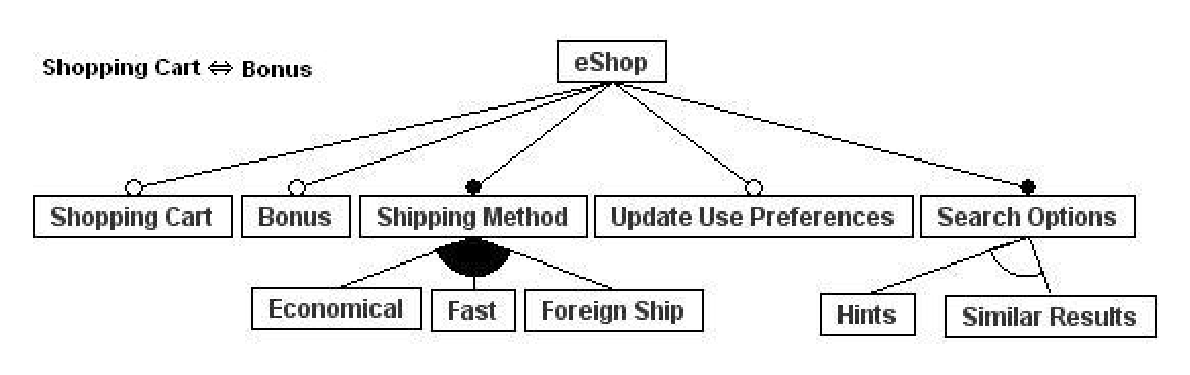
\includegraphics[scale=0.45]{img/eShop-FM.eps}
   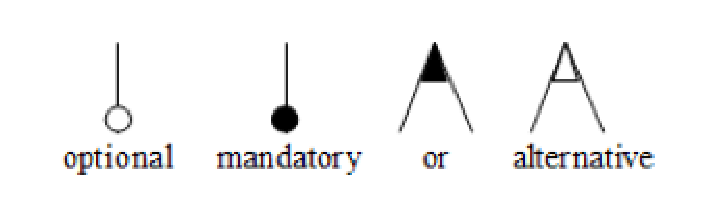
\includegraphics[scale=0.40]{img/fm-notation.eps}
  \caption{eShop feature model.}
  \label{fig:eshop-fm}
  \end{center}
\end{figure}


%Other approaches are based on use case extensions~\cite{jacobson-reuse-book}, not explored here since they
%require that one use case extension must be defined for each variant. This can result in a huge
%number of use cases that is not suitable for managing activities.


Figure~\ref{fig:pluss-01} depicts the \emph{Buy Product} scenarios written in
the PLUSS notation. Notice that a single artifact is used to represent all valid
configurations related to this scenario, mixing common behavior, variant
behavior, and configuration information (feature selection inside square
brackets). For example, steps 1(a) and 1(b) are never performed together. They
are alternative steps: Step 1(a) will be present only if the \emph{Shopping
Cart} feature is selected, otherwise Step 1(b) will be present. In a similar
way, we have to choose between options (a) and (b) for Step 2 (depending whether
the \emph{Bonus} feature is selected or not). Finally, Step 6 is optional and
would be present only if the feature \emph{Update User Preference} was selected.

As a consequence, since all possible variants are described in the same
artifact, PLUSS approach presents difficulties for understanding the behavior
of specific products, because all possible variants are described in the same artifact. 
Moreover, such tangling between \emph{common} and
\emph{variant} behavior results in maintainability issues: introducing a new product variant
requires changes in several points of existing scenarios. For example, including a
\emph{B2B Integration} feature, which allows the integration between partners in
order to share their warehouses, might change the specification of the \emph{Buy
Product} scenario, enabling the search for product availability in remote
warehouses (a new variant for Step 1) and updating a remote warehouse when the
user confirms the purchase (a new variant for Step 5). Moreover, the inclusion of
this new optional feature also changes the specification of the \emph{Search for
Products} scenario (the search might also be remote). The effort
needed to understand and evolve a product line increases, since the
specification of certain features is scattered through several scenarios,
and each scenario describes several configurations.

% In the PLUSS notation, this kind of relationship between
% features and scenarios is scattered throughout different scenarios.


\begin{figure}[h]
\begin{center}
\begin{scriptsize}
  \texttt{
  \begin{tabular}{|p{0.2in}|p{1.3in}|p{1.3in}|}
   \hline
	Id    & User Action & System Response \\ \hline \hline
       1(a) &Select the checkout option. \mbox{[ShoppingCart]}& Present the
       items in the shopping cart and the amount to be paid. The user can remove
       items from shopping cart. \\  \hline 1(b) & Select the buy product
       option. \mbox{[not ShoppingCart]} & Present the selected product. The
       user can change the quantity of items that he wants to buy. Calculate
       and show the amount to be paid. \\  \hline 2(a) & Select the confirm option. [Bonus]& Request bonus and payment information. \\  \hline 2(b) & Select the confirm option. [not Bonus]& Request payment
       information. \\  \hline 3     & Fill in the requested information and select the proceed option. & Request the shipping method and address.\\  \hline 4     & Select the \$ShippingMethod\$, fill in the destination address and select the proceed option. & Calculate the shipping costs. \\  \hline
       5     & Confirm the purchase. & Execute the order and send a request to the Delivery System in order to dispatch the products. \\  \hline
       (6)     & Select the close session option. \mbox{[Update User
       Preferences]} & Register the user preferences.\\  \hline
  \end{tabular}
  }
\end{scriptsize}
\caption{Buy Products scenarios using the PLUSS notation.}
\label{fig:pluss-01}
\end{center}
\end{figure}



% Section~\ref{sec:evaluation} presents a quantitative study regarded to the PLUSS'
% maintanability issues.

% For example, including a \emph{B2B Integration}
% feature, which allows the integration between partners in order to share their warehouses, might change the specification of the \emph{Buy
% Product} scenario, enabling the search for product availability in remote
% warehouses (a new variant for Step 1) and updating a remote warehouse when the
% user confirms the purchase (a new variant for Step 5). Moreover, the inclusion of
% this new optional feature also changes the specification of the \emph{Search for
% Products} scenario (the search might also be remote). In summary, since the
% behavior of certain features may be spread among several specifications and each
% specification might describe several variants, the effort needed to understand
% and evolve the product line might increase.


Differently, PLUC introduces special tags for representing variation points in
use case scenarios. For example, the VP1 tag in Figure~\ref{fig:pluc-01}, which also
describes the \emph{Buy Products} scenario, denotes a variation point that might
assume the values ``\emph{checkout}'' or ``\emph{buy product}'', depending on
which product is being configured. For each \emph{alternative} or
\emph{optional} step, one tag must be defined. The actual value of each tag is specified in the
\emph{Variation Points} section of a scenario specification.

\begin{figure}[h]
\begin{center}
\begin{scriptsize}
  \texttt{
  \begin{tabular}{{|p{0.05in}p{3in}|}}
  \hline
  & {\bf Buy Products Scenario} \\
  & {\bf Main Flow} \\
  01 & Select [VP1] option \\
  02 & [VP2] \\
  03 & Select the confirm option \\
  04 & [VP3] \\
  05 & Fill in the requested information and select the proceed option \\
  06 & Request the shipping method and address \\
  07 & Select the [VP4] shipping method, fill in the destination address and select the proceed option \\
  08 & Calculate the shipping costs. \\
  09 & Confirm the purchase. \\
  10 & Execute the order and sends a request to the Delivery System in order to dispatch the products \\
  11 & Select the close section option. \\
  12 & \{[VP5] Register the user preferences.\} \\  & \\
  & {\bf Products definition: } \\ & VP0 = (P1, P2) \\ & \\
  & {\bf Variation points: } \\
  &  VP1 =  if (VP0 == P1) then (checkout) \\ & \hspace{0.25in} else (buy product) \\
  & VP2 =  if (VP0 == P1) \\ & \hspace{0.25in}  then (Presents the items in the shopping cart...) \\ & \hspace{0.25in} else (Present the selected product. The user...) \\
  & VP3 =  if (VP0 == P1) \\ & \hspace{0.25in} then ( Requests bonus and payment information.) \\ & \hspace{0.25in} else (Requests payment information.) \\
  & VP4 =  (Economic, Fast) \\
  & VP5 requires (VP0 == P1) \\ \hline
   \end{tabular}
  }
\end{scriptsize}
\end{center}
\caption{Buy Products scenarios using the PLUC notation.}
\label{fig:pluc-01}

\end{figure}

Another kind of tangling occurs in this case. the specification of common and
variant behavior are separate, but both are tangled to the variation points. 
Additionally, SPL members are also described using the same tag notation (see the
\emph{Products Definition} section in Figure~\ref{fig:pluc-01}). There is no
explicit relationship between product configurations and feature models. In the
example, two products (P1 and P2) are defined. The first product is configured by
an implicit selection of the \emph{Shopping Cart}, \emph{Bonus}, and \emph{Update
User Preferences} features; in contrast to the second product that is not
configured with these features.


As the values of alternative and optional variation points are computed based on
the defined products, instead of specific features, the inclusion of a new member
in the product line might require a deep review of the \emph{Variation Points}
section in many scenarios. Moreover, since the variation points and the product
definitions are spread among several scenario specifications, it is hard and time
consuming to keep consistent the relationships between them. Finally, the same
definitions (product configuration and variation points) often are useful to manage variabilities in other artifacts, such as design and source code. As a consequence, this approach
requires the replication of such definitions in different SPL views --- when the
SPL evolves, changes are propagated throughout many artifacts.


In conclusion, both PLUSS and PLUC do not present a clear separation between
variability assets and scenario specifications, which compromises the
evolution of a SPL. Besides that, both approaches rely on simple
variability techniques: filtering optional steps in scenarios, or syntactic
changes of tag values based on product definition. In this sense, according to the terminology
presented in~\cite{Kastner:2008aa}, they can be classified as \emph{annotated
techniques}, which are not suitable for modularizing the crosscutting nature of certain
features, have poor legibility, and lead to lower
maintainability~\cite{Alves:2006aa}. 

% For this reason, Pohl et al. argued that the
% variability management concern should be separated from the other SPL
% assets~\cite{Pohl:2005aa}. However, besides the use of independent models for
% representing the variability concern, it is also necessary concrete descriptions
% of the composition processes used to generate specific products.


% this case, in order to support the automatic derivation of product specific
% artifacts, it is necessary not only to have a more precise definition of each
% language used to describe product line artifacts and the variability management
% concern, but also to formalize the weaving processes used to combine them.
%
% The
% PLUSS and PLUC approaches fail in this direction, since Eriksson et al. defines
% the metamodel of PLUSS notation~\cite{eriksson-splc-2005}, but do not describe
% which languages and processes are used for relating use case scenarios to feature
% models. Likewise, although Fantechi et al. describe the formal semantics of
% PLUC~\cite{fantechi-splc-2004}, this approach does not separate variability
% management from use case scenarios.

% Next section describes our approach, named as Scenario Variability as
% Crosscutting Mechanisms (SVCM), which deals with scenario variability
% management by means of the composition of different artifacts. A key
% characteristic found in SVCM is that each involved artifact has a clear and
% specific contribution to the SPL engineering.

% Although in this paper we are focus on use
% case scenarios, the idea of separating product line artifacts from variability
% management (using feature models, product configurations, and configuration
% knowledge) is also applied to other SPL views.
% -------------------------------------------------------------------------
% Section: Modeling the Variability Mechanisms
% ------------------------------------------------------------------------
\section{SVCM Approach}
\label{sec:models}

To solve the problems mentioned in the previous section, we introduce now our
approach for modeling variabilities in use case scenarios, which was named as
\emph{Scenario Variability as Crosscutting Mechanisms} (SVCM). It improves the
separation of concerns between variability management and scenario specifications, dealing with scenario variability as a composition of the
following artifacts: SPL use case model, feature model, product configuration,
and configuration knowledge. 

Motivated by the Masuhara and Kiczales
framework~\cite{Masuhara:2003aa}, our approach for \textbf{scenario variability
management} is based on a weaving process that takes as input the aforementioned
specifications, which crosscut each other with respect to the resulting product
specific use case model (Figure~\ref{fig:weave-process}). Combining these input
languages, it is possible to represent the sources of variability that we are
interested in: \emph{variation in function}, \emph{variation in data}, and
\emph{variation in control flow}~\cite{Bachmann:2001aa}.

\textcolor{red}{
We detail our approach showing how it
can be used to specify the motivating example... 
after that we describe the semantics of our approach using a slight
customization of the MK...
}

\begin{figure}[htb]
 \begin{center}
  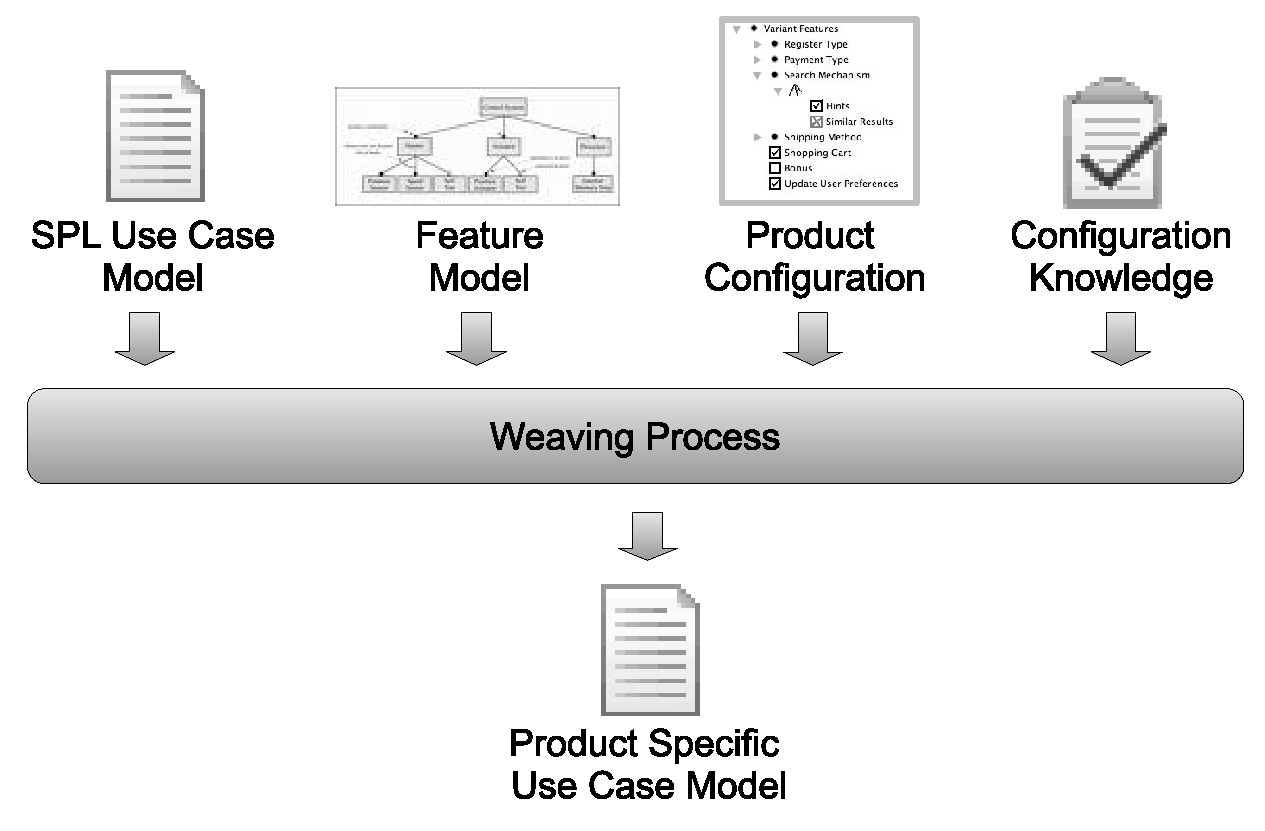
\includegraphics[scale=0.30]{img/weave-process2.eps}
  \caption{Overview of our weaving process.}
  \label{fig:weave-process}
  \end{center}
\end{figure}

\subsection{SVCM example}
\label{sub:running}

In order to explain how the input models (Figure~\ref{fig:weave-process})
crosscut each other with respect to the final product, in this section we
present a running example of our approach. Several artifacts of each input model
are shown; mentioning the contribution of these models to the whole weaving
process.

\subsubsection{Feature model}

Feature models have an important contribution to our
weaving process, since they are used for checking if a product
configuration is a valid member of the product line. It is important to note
that we are not proposing a new notation for feature modeling. Here we
only present the features required (Figure~\ref{fig:eshop-fm-re}) for
understanding the SVCM example.

\begin{figure}[h]
 \begin{center}
  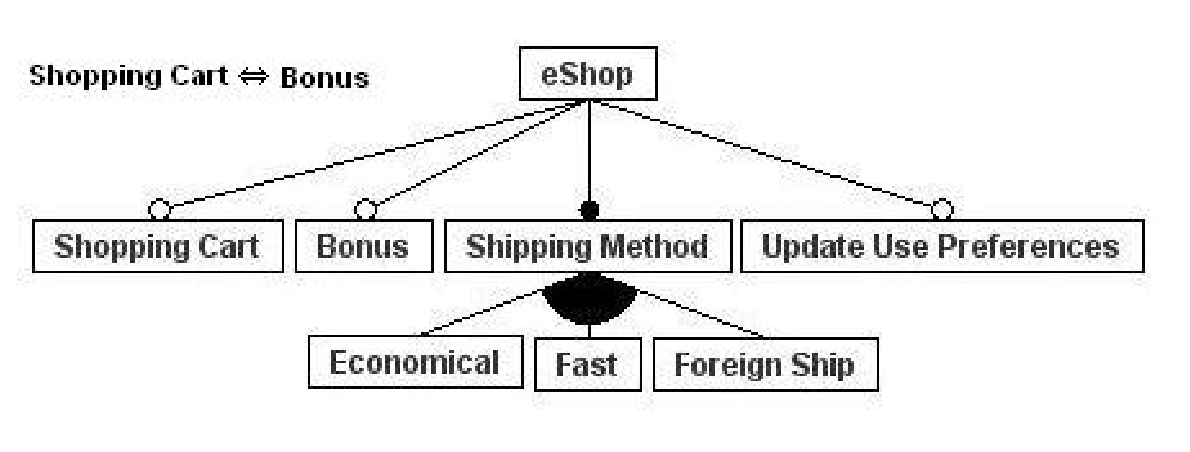
\includegraphics[scale=0.40]{img/eShop-FM2.eps}
   \caption{Subset of eShop feature model.}
  \label{fig:eshop-fm-re}
  \end{center}
\end{figure}

Based on the feature model of Figure~\ref{fig:eshop-fm-re}, the \emph{Shopping
Cart}, \emph{Bonus} and \emph{Update User Preferences} features are optional; on
the other hand, the \emph{Shipping Method} feature is mandatory and all products
have to be configured with at least one of its child. Additionally, the
restriction $Shopping\ Cart\ \Leftrightarrow\ Bonus$ states that all
products configured with the shopping cart feature must also be configured with
the bonus feature. More details about feature modeling can be found
elsewhere~\cite{Gheyi:2006aa,Czarnecki:2000aa}.


\subsubsection{SPL use case model}

This artifact defines scenarios that describe the expected behavior of the SPL's
members. Scenarios might be optional, have parameters, and change (advice) the
behavior of other scenarios. A use case model is composed by \emph{use cases} and
\emph{aspectual use cases}. A use case has a name, a description and a list of
scenarios, which consist of a sequence of steps (pairs of \emph{User action x
System response}). An aspectual use case has a name and a list of advice, which
can be used to extend the behavior of existing scenarios. Differently from
PLUSS and PLUC, our proposed scenarios are not enriched with alternative steps,
product definition, and information related to configurability.  

In this SVMC example, we consider the following scenarios and advices:

{\bf Proceed to Purchase:} this mandatory scenario
(Figure~\ref{fig:proceed-to-checkout}) specifies the common behavior that is
required for confirming a purchase. Instances of the product line must be
configured with this scenario. Notice that a parameter
\emph{ShippingMethod} is referenced in Step P2. This parameter (notation
also supported in PLUSS and PLUC) allows the reuse of the \emph{Proceed to
Purchase} scenario for different configurations of \emph{shipping method}. 

\begin{figure}[h]
\begin{scriptsize}
  \texttt{
   \begin{tabular}{l}
   	 {\bf Id: SC01} 	\\
     {\bf Description:} Proceed to purchase\\
   \end{tabular}
  \begin{center}
  \begin{tabular}{|p{0.1in}|p{1.4in}|p{1.4in}|}
   \hline
       Id & User Action  & System Response \\ \hline \hline
       P1 & Fill in the requested information and select the proceed option.  & Request the shipping method and address.\\  \hline
       P2 & Select one of the available ship methods (\mbox{<SM>}),
       fill in the destination address and proceed. & Calculate the shipping costs. \\  \hline P3 & Confirm the purchase. & Execute the order and send a request to the Delivery System to dispatch the products.
       \mbox{[RegisterPreference]} \\  \hline
  \end{tabular}
  \end{center}
  }
\end{scriptsize}
\caption{Proceed to purchase scenario.}
\label{fig:proceed-to-checkout}
\end{figure}

{\bf Buy Product:} this advice (Figure~\ref{fig:buy-product-scenario}) enables a
customer to buy specific goods from an on-line shopping store. It is only
available in the product line members that are {\bf not} configured with the
\emph{Shopping Cart} and \emph{Bonus} features. Differently from the PLUSS
approach, which directly relates alternative and optional steps to features, in
our approach this kind of information is represented in a distinct artifact: the
configuration knowledge. The effect of this advice is to introduce an optional behavior {\bf
before} the join points identified in its \emph{pointcut} clause. In this case,
the Step P1 defined in the \emph{Proceed to Purchase} scenario.

\begin{figure}[h]
\begin{scriptsize}
  \texttt{
   \begin{tabular}{l}
   	 {\bf Id: ADV01} 	\\
     {\bf Description:} Buy a specific product\\
     {\bf Before:}  P1
   \end{tabular}
  \begin{center}
  \begin{tabular}{|p{0.1in}|p{1.4in}|p{1.4in}|}
   \hline
       Id & User Action  & System Response \\ \hline \hline
       B1 & Select the buy product option.  & Present the selected product. The user can change the quantity of items he wants to buy. Calculate and show the amount to be paid. \\  \hline
       B2 & Select the confirm option. &  Request payment information. \\  \hline
    \end{tabular}
  \end{center}
  }
\end{scriptsize}
\caption{Buy product advice.}
\label{fig:buy-product-scenario}
\end{figure}

{\bf Buy Products with Shopping Cart and Bonus:} this advice
(Figure~\ref{fig:buy-product-changing-flow}) allows purchasing products
that have been previously added to a customer shopping cart. It extends the
behavior of the \emph{Proceed to Purchase} scenario by introducing the specific
behavior required by the \emph{Shopping Cart} and
\emph{Bonus} features. Therefore, this advice is required by products that
are configured with both \emph{Shopping Cart} and \emph{Bonus} features.

\begin{figure}[h]
\begin{scriptsize}
  \texttt{
   \begin{tabular}{l}
   	 {\bf Id: ADV02} 	\\
     {\bf Description:} Buy products using a shopping-cart\\
     {\bf Before:} P1
   \end{tabular}
  \begin{center}
   \begin{tabular}{|p{0.1in}|p{1.4in}|p{1.4in}|}
   \hline
       Id & User Action & System Response \\ \hline \hline
       C1 & Select the checkout option.  & Present the items in the shopping cart and the amount to be paid. The user can remove items from the shopping cart. \\  \hline
       C2 & Select the confirm option. & Request bonus and payment information. \\  \hline
  \end{tabular}
  \end{center}
  }
\end{scriptsize}
\caption{Buy products with shopping cart advice.}
\label{fig:buy-product-changing-flow}
\end{figure}

As shown in Section~\ref{sec:problem}, PLUSS and PLUC represent all valid
configurations of a scenario in a single artifact. Using our approach, we were
able to separate the common behavior required to confirm a purchase (the base
scenario \emph{Proceed to Purchase}) from its variants, specified in the
\emph{Buy Product} and \emph{Buy Product with Shopping Cart} advices. This allows
our specifications to evolve according to the \emph{Open-Closed}
principle~\cite{Meyer:2000aa}. In our approach, introducing new product variants
require more extensions than changes to the base scenarios. {\bf Search for
Products:} this mandatory scenario (Figure~\ref{fig:search-products-flow}) allows
the user to search for products. In order to save space, we only present Step S3,
which performs a search based on the input criteria. This step is annotated with
the mark \mbox{{\bf [RegisterPreference]}}, exposing it as a possible extension
point for the behavior of \emph{Register User Preferences}
(Figure~\ref{fig:register-preferences-flow}). The same annotation was assigned to
the Step P3 of \emph{Proceed to Purchase} (Figure~\ref{fig:proceed-to-checkout}).
Such annotations can be referenced by advices, and were proposed as an attempt to
reduce the problem of fragile pointcuts. \textcolor{red}{We believe that,
similarly to the use of annotations, introducing semantic based mechanisms to
compose scenarios~\cite{Chitchyan:2007aa} does not require significant changes to
the SVMC weaving process.}


\begin{figure}[ht]
\begin{scriptsize}
  \texttt{
   \begin{tabular}{l}
   	 {\bf Id: SC02} 						\\
     {\bf Description:} Search for products. \\
   \end{tabular}
  \begin{center}
   \begin{tabular}{|p{0.1in}|p{1.4in}|p{1.4in}|}
   \hline
       Id & User Action &  System Response \\ \hline \hline
       \ldots & \ldots  & \ldots \\  \hline
       S3 & Inform the search criteria. &  Retrieve the products that satisfy the search criteria. Show a list with the resulting products. [RegisterPreference] \\  \hline
  \end{tabular}
  \end{center}
  }
\end{scriptsize}
\caption{Search for products scenario.}
\label{fig:search-products-flow}
\end{figure}

{\bf Register User Preferences:} this advice updates the user preferences based
on the user's history of searches and purchases. Its behavior can be started {\bf
after} any step assigned to the {\bf [RegisterPreference]} (see the
\emph{pointcut} clause) annotation and is available in products that are
configured with the \emph{Update User Preferences} feature.

\begin{figure}[h]
\begin{scriptsize}
  \texttt{
   \begin{tabular}{l}
   	 {\bf Id: ADV03} 	\\
     {\bf Description:} Register user preferences.\\
     {\bf After}: [RegisterPreference] \\
   \end{tabular}
  \begin{center}
   \begin{tabular}{|p{0.1in}|p{1.4in}|p{1.4in}|}
   \hline
       Id & User Action &  System Response \\ \hline \hline
       R1 & - &  Update the preferences based on the search results or purchased items. \\  \hline
  \end{tabular}
  \end{center}
  }
\end{scriptsize}
\caption{Register user preferences.}
\label{fig:register-preferences-flow}
\end{figure}

In this example, we described several scenarios as being optional or
mandatory. It is important to observe that, in our approach, this kind of
information is not specified in scenario documents. Actually, it is necessary to
consider the relationships between scenarios and features in order to realize
which configurations require a specific scenario. As we explained at the
beginning of this section, each artifact (feature model, product configuration,
configuration knowledge, and use case model) provides a specific contribution to
the definition of a SPL's member.


\subsubsection{Product configuration}\label{subsub:pc}

This artifact identifies a specific SPL member, which is characterized by a valid
configuration of features. Each product configuration should conform to a feature
model (the selected features should obey the feature model relationships and
constraints). For the \emph{eShop} example, two possible configurations are
presented in Figure~\ref{fig:product-config-01-02}. We represent these configurations as a
tree, highlighting which features were selected. Such a representation was
created using the \emph{Feature Modeling Plug-in}~\cite{Czarnecki:2004aa}


 \begin{figure}[h]
 \begin{center}
  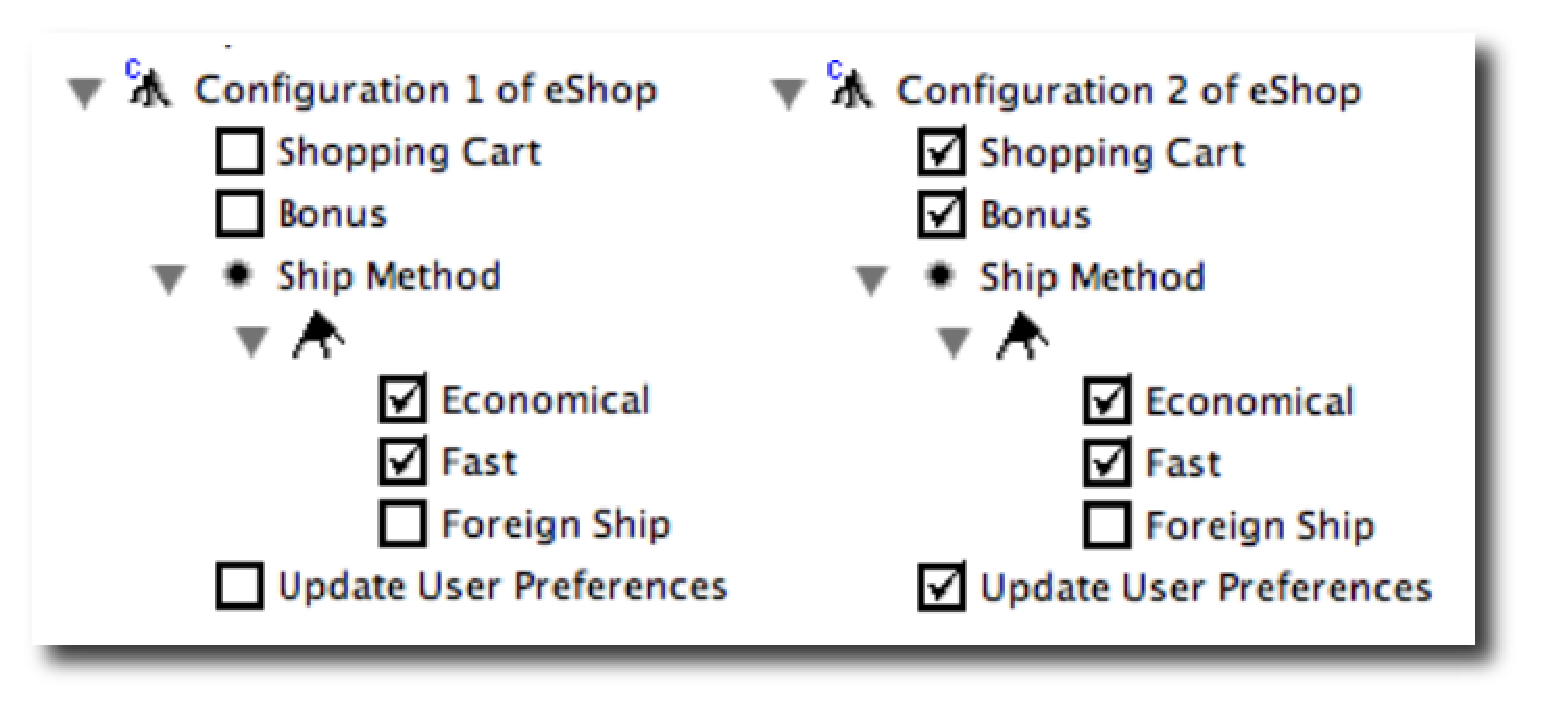
\includegraphics[scale=0.33]{img/pc-04.eps}
   \caption{Examples of product configurations.}
  \label{fig:product-config-01-02}
  \end{center}
\end{figure}

% \begin{figure}[htb] \centerline{
% \mbox{
\includegraphics[scale=0.4]{img/pc-01.eps}}
% \mbox{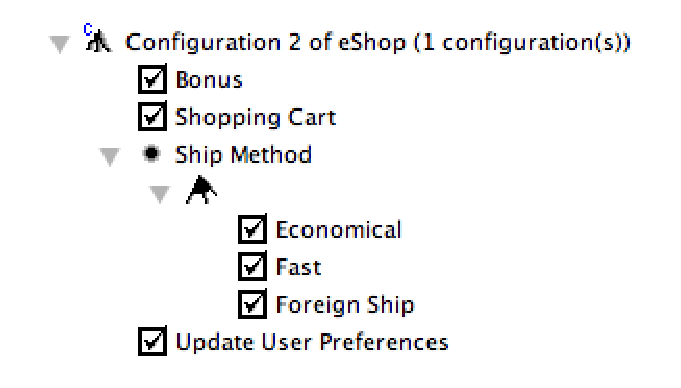
\includegraphics[scale=0.4]{img/pc-02.eps}} } \nocaptionrule
% \caption{Examples of product configurations.} \label{fig:product-config-01-02}
% \end{figure}

The first configuration (on the left side of the
Figure~\ref{fig:product-config-01-02}) defines a product that has no support for
\emph{Shopping Cart}, \emph{Bonus} and \emph{Update User Preferences}.
Additionally, it supports only the economical and fast shipping methods. The
second configuration is more complete, being configured with the features
\emph{Shopping Cart}, \emph{Bonus}, and \emph{Update User Preferences}.

In PLUC, product configurations are scattered through existing scenarios, and
are not explicitly related to features. As discussed in
Section~\ref{sec:problem}, even simple changes in the configuration model might
require a deep review of existing scenarios. 

The set of features selected to a specific product (represented as a product
configuration) identifies which actions must be performed to
generate the corresponding SPL member. In order to do that, the configuration
knowledge (exemplified in what follows) relates feature expressions to such
actions. 

\subsubsection{Configuration knowledge}

This artifact is represented as a list of configuration items, which relates
feature expressions (written in propositional logic) to the actions used for
generating specific product. Therefore, the configuration knowledge allows,
during product engineering, the automatic configuration of SPL assets.
Table~\ref{tab:eshop-ck} presents the configuration
knowledge for the running example, enforcing that


\begin{itemize}
\item Both \emph{Proceed to Purchase} (SC01) and \emph{Search for Products}
(SC02) scenarios are mandatory, since their selection is related to the
(mandatory) root feature of the \emph{eShop} product line;

\item The \emph{Buy Product} advice (ADV01) is used in the composition of
products that do not have been configured with both \emph{Shopping Cart} and \emph{Bonus}
features--- if both features were selected for a product, it would be configured
with the \emph{Buy Product with Cart} advice (ADV02). Remember that there is a
mutual dependency between \emph{Shopping Cart} and \emph{Bonus} features. As a
consequence, no product can be configured with just one of them;

\item The \emph{Register User Preferences} advice (ADV03) is not used in a
product composition unless the \emph{Update User Preferences} feature has been
selected; and

\item References to the ``SM'' parameter are bound to the
selected alternatives of the \emph{Shipping Method} feature.

\end{itemize}


\begin{table}[htb]
\begin{small}
\begin{tabular}{|lp{1.4in}|}
\hline
Feature Expression  						& Actions					 \\ \hline

eShop										& select scenario {\bf SC01} \\
											& select scenario {\bf SC02} \\	\hline 
{\bf not} (Shopping Cart {\bf and} Bonus) 	& evaluate advice {\bf ADV01} \\
\hline (Shopping Cart {\bf and} Bonus) 		& evaluate advice {\bf ADV02} 	\\
\hline Update User Preferences 				& evaluate advice {\bf ADV03} \\ \hline
Shipping Method								& bind parameter {\bf SM}\\ \hline
								
\end{tabular}
\end{small}
\caption{Example of configuration knowledge}
\label{tab:eshop-ck}
\end{table}

Three different actions are used in the configuration knowledge shown in
Figure~\ref{tab:eshop-ck}: \emph{select scenario},
\emph{evaluate advice}, and \emph{bind parameter}. Using the terminology
proposed by Bachmann et al.~\cite{Bachmann:2001aa}, the first weaver deals with
the source of variability named as \emph{variation in function}; the second one
deals with \emph{variation in control flow}; and the last one deals with
\emph{variation in data}. The next section describes a modeling framework 
for representing the semantics of these weavers as crosscutting mechanisms.

Figure~\ref{fig:resulting-purchase} depicts the resulting scenario related to
the purchasing behavior, after evaluating the configuration knowledge of
Table~\ref{tab:eshop-ck}, and considering the second product of
figure~\ref{fig:product-config-01-02}.


\begin{figure}[h]
\begin{scriptsize}
   \texttt{
   \begin{center}
    \begin{tabular}{|p{1.45in}|p{1.45in}|} \hline
       User Action  & System Response \\ \hline \hline
       Select the checkout option.  & Present the items in the shopping
       cart and the amount to be paid. The user can remove items from the
       shopping cart. \\ \hline
       Select the confirm option. & Request bonus and payment information. \\ \hline
       Fill in the requested information and
       select the proceed option.  & Request the shipping method and address.\\ \hline
       Select one of the available ship methods {\bf (Economical, Fast)}, fill
       in the destination address and proceed. & Calculate the shipping
       costs.\\ \hline
       Confirm the purchase. & Execute the order and send a
       request to the Delivery System to dispatch the products. \\ \hline
 	   - &  Update the preferences based on the search results or purchased
 	   items. \\ \hline
    \end{tabular}
   \end{center}
   }
\end{scriptsize}
\caption{Register user preferences.}
\label{fig:resulting-purchase}
\end{figure}		

There is no artifact similar to our configuration knowledge in
PLUSS and PLUC approaches. As a consequence, introducing new variants of existing 
features in these techniques usually propagates changes throughout many
scenarios. Actually, this artifact is responsible for enforcing a clear
separation between variability management and scenario specifications.

%=================================================================
% Semantica do configuration knowledge
%=================================================================
% \begin{figure*}[hbt]
%  \begin{code}
%   (|->) :: a -> b -> (a,b) -- just a 'syntactic sugar' to build pairs
%   l |-> r = (l,r)
% 
%   conf1 = Configuration (``eShop'' |-> selectScenarios[``SC01'', ``SC02''])
%   conf2 = Configuration ('Not' (``ShoppingCart'' 'And' ``Bonus'') |-> evaluateAdvice[``ADV01''])
%   conf3 = Configuration (``ShoppingCart'' 'And' ``Bonus'' |-> evaluateAdvice[``ADV02''])
%   conf4 = Configuration (``UpdateUserPreferences'' |-> evaluateAdvice[``ADV03''])
%   conf5 = Configuration (``ShipMethod'' |-> bindParameter(``ShipMethod'', `ShipMethod''))
%   ...
% 
%   ck = [conf1, conf2, conf3, conf4, conf5]
%  \end{code}
% \caption{eShop configuration knowledge}
% \label{fig:ck-running-example}
% \end{figure*}
% 
% We can reason about the effect of evaluating a configuration knowledge
% by means of trace models, defined to our context as:
% 

% 
% \begin{definition}
% A trace model is the set of valid sequences of events
% computed from the product scenarios. Events are labeled as the step ids of a
% scenario. The trace model for a scenario $s$ is given by:.
% \end{definition}
% 
% \begin{code}
% traceModel s = traces (steps s)
% where
%   traces [] = [[]]
%   traces (x:xs) = [] : (stepId x) ^ (traces (xs))
% 
% (^) :: (a -> [[a]]) -> [[a]]
% x ^ y = [ x:e | e <- y ]
% \end{code}
% 
% For instance, Table~\ref{tab:ck-evaluation} presents the resulting trace models,
% after evaluating each configuration item of Figure~\ref{fig:ck-running-example}
% and considering the second product represented in
% Figure~\ref{fig:product-config-01-02}. Notice that the trace model of an empty
% product is the set with just one element: the empty sequence of events (not
% represented in Table~\ref{tab:ck-evaluation}).
% 
% \begin{table}[hbt]
%   \begin{tabular}{{||m{0.3in} m{0.1in} p{0.05in} l||}}
%   	\hline
%  	Config 		  & Eval		 & & Trace Model  \\  \hline 	
%  	
%  	$conf1$		  & True	     & & \parbox[t]{2.4in} {
%  									 \raggedright
%  									 <>, <P1>, <P1,P2.sm>, <P1,P2.sm,P3>,
%  									 <S1>, <S1,S2>, <S1,S2,S3> \\
%  								    } 									
%     								\\ \hline
%     $conf2$		  & False	   & & \parbox[t]{2.4in} {
%  								   \raggedright
%  									 <>, <P1>, <P1,P2.sm>, <P1,P2.sm,P3>,
%  									 <S1>, <S1,S2>, <S1,S2,S3> \\
%  								  }
%  								 \\ \hline 										
% 	$conf3$		  & True	   & & \parbox[t]{2.4in} {
%  								   \raggedright
%  									 <>, <C1>, <C1,C2>, <C1,C2,P1>,
% 							         <C1,C2,P1,P2.sm>, <C1,C2,P1,P2.sm,P3>,
%  								     <S1>, <S1,S2>, <S1,S2,S3> \\
%  								   } 								
%  								 \\ \hline
% 	$conf4$		  & True	   & & \parbox[t]{2.4in} {
%  								   \raggedright
% 	                                <>, <C1>, <C1,C2>, <C1,C2,P1>,
% 							        <C1,C2,P1,P2.sm>, <C1,C2,P1,P2.sm,P3>,
% 							        <C1,C2,P1,P2.sm,P3,R1>,
%  								    <S1>, <S1,S2>, <S1,S2,S3>,
%  								    <S1,S2,S3,R1> \\
%  								   }   	
%  								 \\ \hline
% 	$conf5$		  & True	   & & \parbox[t]{2.4in} {
%  								   \raggedright
% 									<>, <C1>, <C1,C2>, <C1,C2,P1>,
% 							     <C1,C2,P1,P2.(Economical,Fast)>,
% 							     <C1,C2,P1,P2.(Economical,Fast),P3>,
% 							     <C1,C2,P1,P2.(Economical,Fast),P3,R1>
%  								 <S1>, <S1,S2>, <S1,S2,S3>,
%  								 <S1,S2,S3,R1> \\   	 							
%  								 }
%  								 \\ \hline	 						  	
%  				
%    \end{tabular}
% \caption{The effect of evaluating configuration items}
% \label{tab:ck-evaluation}
% \end{table}

%=================================================================
%=================================================================




% In what follows, we describe a high level view of the weaving process that
% combines the input languages in order to manage scenario variability.  Then, in
% Section~\ref{sub:modeling-framework} we formally present its semantics in terms
% of our modeling framework.

% \subsubsection{Weaving process}
%
% The weaving process represented in Figure~\ref{fig:weave-process} is responsible for performing the following activities:
%
% {\bf Validation activity:} This activity is responsible for checking if a product configuration is a valid instance of the feature model. If the product configuration is
% valid (it conforms to the relationship cardinalities and constraints of the feature model), the process might proceed.
%
% {\bf Product derivation activity:} This activity takes as input a (valid) product configuration and a configuration knowledge.
% Each feature expression of the configuration knowledge is checked against the product configuration. If the expression
% is satisfied, the related scenarios are assembled as the result of this activity. For the running example,
% Table~\ref{tab:assembled-scenarios} shows the assembled scenarios for the configurations depicted in Figure~\ref{fig:product-config-01-02}.
%
% \begin{table}[h]
% \begin{center}
% \caption{Assembled scenarios} \label{tab:assembled-scenarios}
% \begin{tabular}{ll}
%    \hline\noalign{\smallskip}
%   {\bf Configuration} & {\bf Assembled scenarios} \\
%    \noalign{\smallskip}
%    \hline
%    \noalign{\smallskip}
%     Configuration 1\hspace{15pt} & Proceed to Purchase \\
%                                                    & Search for Products \\
%                                                    & Buy a Product \\
%                              			  & \ldots \\
%    Configuration 2                        & Proceed to Purchase \\
%                              			  & Search for Products	 \\
% 			                           & Buy Products with Cart \\
%                                                    & Register User Preferences \\
%                              & \ldots       \\
%   \hline
% \end{tabular}
% \end{center}
% \end{table}
%
%  {\bf Scenario composition activity:} This activity is responsible for composing the scenarios assembled for a specific product configuration.
% Therefore, the resulting scenarios of the previous activity, which crosscut each other based on the \emph{From step} and \emph{To step clauses}, are woven. The
%  result is a use case model with complete paths (all \emph{From step} and \emph{To step} clauses are resolved).
%
% %  or a trace model (a set of all valid sequences of events extracted from the complete paths).
%
% The complete path is a high level representation, which uses the same constructions of the use case model (scenarios), and is illustrated here as a graph, where each node is labeled with a step id. For example, Figure~\ref{fig:complete-paths} depicts the complete paths for the first and second configurations of our running example. In the left side of the figure,  the composition of \emph{Buy a Product} with \emph{Proceed to Purchase} (branch labeled as B1, B2, P1, P2, P3) and \emph{Search for Product} (branch labeled as S1, S2, S3) scenarios are presented. Contrasting, on the right side of the figure, the results of this activity is presented for the second configuration. In this case, steps B1 and B2 have been replaced by steps V1 and V2 (because \emph{Shopping Cart} and \emph{Bonus} features are selected) and the step  R1 is introduced after steps P3 and S3 (because \emph{Update User Preferences} is selected in this configuration).
%
% %=====================
% % Trace model discussion
% %=====================
%
% %Instead, the trace model can be seen as a low level representation of the use case model. Such notation has a well defined semantic and might
% %be used for model checking and test case generation. Such applications of the trace model are beyond the scope of this paper. More information
% %can be found elsewhere\cite{csp-hoare,csp-roscoe,cfeitosa-sbmf-2006}. Here, the trace model is useful for implementing the last activity of our weave process, binding parameters, and
% %represents all possible sequences of events in a specific product configuration.
%
% %For instance, the trace model for the first configuration is the set of sequences:
%
% %\begin{small}
% %\begin{tabular}{rlc}
% %$Trace_{C1}$ = & \{<>, <idle>, <idle, 1S>, <idle, 1S, 2S>, \\
% %                    & <idle, 1S, 2S, 3S>,  <idle, 1S, 2S, 3S, end>, \\
% %                    & <idle, 1M>, <idle, 1M, 2M>, \ldots, \\
% %                    & <idle, 1M, 2M, 3M, 4M.ShipMethod, 5M, end> \}
% %\end{tabular}
% %\end{small}
%
% %========================
%
% % \begin{figure}[bth]
% % \begin{center}
% % \begin{tiny}
% % \begin{xy}
% % \xymatrix@R=10pt{
% % & *++[o][F-]{idle} \ar[r]\ar[d] & *++[o][F-]{B1} \ar[d]	& *++[o][F-]{idle} \ar[r]\ar[d] & *++[o][F-]{V1} \ar[d] 		\\
% % & *++[o][F-]{S1} \ar[d]  & *++[o][F-]{B2} \ar[d]           & *++[o][F-]{S1} \ar[d]  & *++[o][F-]{V2} \ar[d] 			\\
% % & *++[o][F-]{S2} \ar[d]  & *++[o][F-]{P1} \ar[d]           & *++[o][F-]{S2} \ar[d]  & *++[o][F-]{P1} \ar[d]			\\
% % & *++[o][F-]{S3} \ar[d]  & *++[o][F-]{P2} \ar[d]           & *++[o][F-]{S3} \ar[d]  & *++[o][F-]{P2} \ar[d] 			\\
% % & *++[o][F-]{end} & *++[o][F-]{P3} \ar[l]                     & *++[o][F-]{R1} \ar[d] & *++[o][F-]{P3} \ar[l]   			\\
% % &                         &                                                    &   *++[o][F-]{end}       &
% % }
% % \end{xy}
% % \end{tiny}
% % \caption{Complete paths represented  as a graph}
% % \label{fig:complete-paths}
% % \end{center}
% % \end{figure}
%
% {\bf Binding parameters activity:}  This activity weaves scenarios and product configurations in order to resolve all scenario parameters.
% For example, step P2 in Figure~\ref{fig:proceed-to-checkout} has a reference
%  to the \emph{ShipMethod} parameter, whose domain values are defined in the product configuration. For instance, in the first configuration depicted in Figure~\ref{fig:product-config-01-02}, the parameter \emph{ShipMethod} might assume the values \emph{Economical} or \emph{Fast}.
% In order to reduce the coupling between scenario specifications and feature model, a mapping is used for relating scenario parameters to features. In fact, this mapping is another input artifact of our modeling framework; but it was not represented in Figure because it was just introduced for avoiding explicit dependences between feature and use case models.
% Next, we introduce the modeling framework used to formally describe the weaving processes just presented.
% %===================
% % Trace model discussion
% %===================
%
% %For each trace that contains a parameterized event (or step), this activity creates a new trace for all of the possible parameter values. Consequently, resolving parameters for the trace $<idle,1M,2M,3M,4M.ShipMethod>$ results in the following sequences:
% %
% %\begin{center}
% %\begin{small}
% %\begin{tabular}{c}
% %<idle,1M,2M,3M,4M.Economical>, \\ <idle,1M,2M,3M,4M.Fast>, \\
% %\end{tabular}
% %\end{small}
% %\end{center}


% ================================= Modeling Framework
% =================================

\subsection{Modeling Framework}\label{sub:modeling-framework}

In this Section we describe the notation proposed to represent variability
management as crosscutting mechanisms. Actually, our notatin is a slight
customization of the \emph{Crosscutting Modeling Framework}, proposed by Masuhara
and Kiczales (the MK framework)~\cite{Masuhara:2003aa}. The goal of the MK
framework is to explain how different \emph{aspect-oriented} mechanisms support
crosscutting modularity. In order to do that, each mechanism is represented as a
three-part description: the related weaving processes take two programs as input,
which crosscut each other with respect to the resulting program or
computation~\cite{Masuhara:2003aa}.

Their requirement for characterizing a mechanism as crosscutting is fulfilled by
our approach, in the sense that different specifications contribute to the
definition of a specific SPL member, as ilustrated in the previous section. As a
consequence, due to its crosscutting nature, the modeling framework proposed
in~\cite{Masuhara:2003aa} is suitable for formalizing variability management
compositions.

As a slight customization of MK work, our modeling framework represents each
weaver as an 6-tuple (Eq.~\ref{eq:tuple} and Table~\ref{tab:tup-01}),
highlighting the contribution of each input language in the composition
processes. We represent each weaver by filling in the six parameters of our
6-tuple representation, by providing a reference implementation for each weaver,
and by stating how elements of the weaver implementation correspond to elements
of the model.

In our modeling framework, the concrete semantics of those weavers (and the
meta-model of the input and output languages) are described using the Haskell
programming language~\cite{Jones:2002aa}. This led to concise descriptions and
kept our model close to the MK work, where their weaving processes are specified
in the Scheme programming language. The choice for Haskell was motivated by
several factors, such as improved readability and our background in the language.
The resulting source code is available at a web site~\cite{SPG:site}.

\begin{equation}
W = \{o, o_{jp}, L, L_{id}, L_{eff}, L_{mod}\},
\label{eq:tuple}
\end{equation}

\begin{table}[h]
\begin{center}
\caption{Modeling framework elements.} \label{tab:tup-01}
\begin{tabular}{|p{0.6in}|p{2.4in}|}
  \hline
  {\bf Element} & {\bf Description} \\
   \hline
  $o$              & Output language used for describing the results of the weaving process \\ \hline
  $o_{jp}$       & Set of join points in the output language \\ \hline
  $L$              & Set of languages used for describing the input specifications \\ \hline
  $L_{ID}(l)$      & Set of constructions in each input language $l$, used for identifying the output join points \\ \hline
  $L_{EFF}(l)$   & For each input language $l$, this element represent the effect of its constructions in the weaving process \\ \hline
  $L_{MOD}(l)$  & Set of modular unities of each input language $l$\\ \hline
  \hline
\end{tabular}
\end{center}
\end{table}

In the next sections we describe the semantics of
our weaving process. For simplicity, this description is explained in three
different parts (\ref{sub:pd-weaver}-- \ref{sub:bind-weaver}); one weaver
description for each source of variability. 

\subsection{Variability in function}\label{sub:pd-weaver}

Variability in function occurs when a particular function might exist in some
products and not in others~\cite{Bachmann:2001aa}. For this source of
variability, a corresponding weaver is responsible for selecting scenarios based
on specific product configurations. Although in this paper we focus only in the
selection of scenarios that should be assembled in specific instances of the SPL,
this weaver can be easily extended for managing variabilities in other kinds of
assets (aiming at selecting design elements, source code, and test cases). 

This weaver is implemented by the function \emph{selectScenarios}
(Figure~\ref{fig:interpreter-vf}). It takes as input the list of \emph{scenario
ids} that should be selected for a specific feature expression,  the \emph{SPL
use case model} (spl), and the $product$ being generated. Then, this function
returns a new configuration of the product, which is refined by each scenario $s$
in the SPL use case model that satisfies the condition $(id\ s) \in\ ids$. In
this case, the configuration knowledge (CK) and the SPL use case model
(UCM) crosscut each other with respect to the list of scenarios added to the
specific SPL member.

\begin{figure}[ht]
\begin{hscode}\SaveRestoreHook
\column{B}{@{}>{\hspre}l<{\hspost}@{}}%
\column{3}{@{}>{\hspre}l<{\hspost}@{}}%
\column{5}{@{}>{\hspre}l<{\hspost}@{}}%
\column{E}{@{}>{\hspre}l<{\hspost}@{}}%
\>[B]{}\Varid{selectScenarios}\;\Varid{ids}\;\Varid{spl}\;\Varid{product}\mathrel{=}{}\<[E]%
\\
\>[B]{}\hsindent{3}{}\<[3]%
\>[3]{}\Varid{addScenarios}\;(\Varid{product},\Varid{scenarios}){}\<[E]%
\\
\>[B]{}\hsindent{3}{}\<[3]%
\>[3]{}\mathbf{where}{}\<[E]%
\\
\>[3]{}\hsindent{2}{}\<[5]%
\>[5]{}\Varid{scenarios}\mathrel{=}[\mskip1.5mu \Varid{s}\mid \Varid{s}\leftarrow (\Varid{splScenarios}\;\Varid{spl}),(id\;\Varid{s})\;\in\;\Varid{ids}\mskip1.5mu]{}\<[E]%
\\
\>[3]{}\hsindent{2}{}\<[5]%
\>[5]{}\Varid{addScenarios}\mathbin{...}{}\<[E]%
\ColumnHook
\end{hscode}\resethooks
\caption{Interpreter for variability in function}
\label{fig:interpreter-vf}
\end{figure}

Figure~\ref{fig:ci-vf} shows the concrete instantiation of the first line of the
\emph{eShop} configuration knowledge (Table~\ref{tab:eshop-ck}), which deals with this
source of variability. Notice that the configuration knowledge
binds the first parameter of \emph{selectScenario} function. Therefore, 
particularly to this weaver, the configuration knowledge contributes to 
the identification of the scenarios that must be added to a specific product.

\begin{figure}[hbt]
\begin{small}
 \begin{hscode}\SaveRestoreHook
\column{B}{@{}>{\hspre}l<{\hspost}@{}}%
\column{E}{@{}>{\hspre}l<{\hspost}@{}}%
\>[B]{}\Varid{c1}\mathrel{=}\Conid{Config}\;(``\Varid{eShop''},\Varid{selectScenarios}\;[\mskip1.5mu ``\Conid{SC01''},``\Conid{SC02''}\mskip1.5mu]){}\<[E]%
\ColumnHook
\end{hscode}\resethooks
\end{small}
\caption{Configuration item for variability in function}
\label{fig:ci-vf}
\end{figure}

The model of the \emph{Variability in Function Weaver}, in terms of the
framework, is shown in Table~\ref{tab:vf-weaver}. The \emph{selectScenarios}
function is used to argue that the model is realizable and
appropriate~\cite{Masuhara:2003aa}. 
We achieve this by matching the model elements to
corresponding parameters and auxiliary functions in the implementation code. 

The input languages
\emph{configuration knowledge} and \emph{SPL use case model} contributes to the
binding of \emph{selectScenarios} parameters. An instance of the SPL use
case model corresponds to the specification of all SPL scenarios. 
Instead, the identification of wich scenarios must be added to a specific
feature expression are documented in the configuration knowledge. Finally, the
\emph{product configuration} specifies which features were selected for a
specific product.

\begin{table}[htb]
\begin{center}
\caption{Model of Product Derivation} \label{tab:vf-weaver}
\begin{tabular}{p{0.6in}p{2.4in}}
   \hline\noalign{\smallskip}
  {\bf Element} & {\bf Description} \\
   \noalign{\smallskip}
   \hline
   \noalign{\smallskip}
   $o$              & Product specific scenarios (list of scenarios) \\
   $o_{jp}$        	& Scenario declarations \\
   $L$              & \{UCM, CK, PC\} \\
   $UCM_{ID}$ 		& SPL scenarios \\
   $CK_{ID}$    	& Feature expressions and scenario IDs\\
   $PC_{ID}$    	& Product specific feature selection \\
   $UCM_{EFF}$ 		& Provides declaration of scenarios \\
   $CK_{EFF}$    	& Identifies actions to be peformed  \\
   $PC_{EFF}$    	& Triggers scenario selection \\
   $UCM_{MOD}$ 		& Scenario \\
   $CK_{MOD}$    	& Each pair $(feature\ expression, actions)$  \\
   $PC_{MOD}$    	& Feature \\
  \hline
  \end{tabular}
\end{center}
\end{table}

The UCM has a greater importance over the other input languages ($UCM_{EFF}$),
since it declares the parts that compose the product specific scenarios (the
output of this weaver process generated by the \emph{selectScenarios} function).

\subsection{Variability in data}\label{sub:bind-weaver}

This kind of variability occurs whenever two or more scenarios share the same
behavior (the sequence of steps) and differ in relation only to values of a same
concept. For instance, Figure~\ref{fig:proceed-to-checkout} depicts the
\emph{Proceed to Purchase} scenario, which can be reused for different kinds of
shipping method. Without this parameterized specification, and aiming, for
example, at automatically generating a test case suite with a good coverage, it
would be necessary to create a scenario for each kind of shipping method. 

%  This weaver takes into consideration \emph{scenario specifications} and
% \emph{product configurations}, which defines the domain values of a parameter.
% Thus, in order to reduce the coupling between scenarios and features, we
% propose a mapping that relate them. A constraint must be obeyed in this
% mapping: features related to parameters must be either an {\bf alternative
% feature} or an {\bf or
% feature}~\cite{gheyi-alloy-06,czarnecki-wsfactory-2005,czarnecki-book}.


Figure~\ref{fig:ri-vd} presents the reference implementation that solves this
kind of variability. The function \emph{bindParameter} takes as input the
identifier of a parameter ($pId$); the identifier of a feature ($fId$); the
product configuration (\emph{pc}), which defines the domain values of
parameters (expressed as a feature selection); the SPL use case model ($spl$);
and the $product$ being generated. Then, it replaces all references to
pId in the $product$ by a suitable representation for the corresponding
configuration. 


For example, if a product is configured with either \emph{Economical} and
\emph{Fast} shipping methods, the result of applying this weaver for
the \emph{Proceed to Purchase} scenario will result in the
representation (\emph{Economical, Fast}) in each place that the parameter
\emph{ShippingMethod} is referred.

\begin{figure}
\begin{hscode}\SaveRestoreHook
\column{B}{@{}>{\hspre}l<{\hspost}@{}}%
\column{3}{@{}>{\hspre}l<{\hspost}@{}}%
\column{5}{@{}>{\hspre}l<{\hspost}@{}}%
\column{E}{@{}>{\hspre}l<{\hspost}@{}}%
\>[B]{}\Varid{bindParameter}\;\Varid{pId}\;\Varid{fId}\;\Varid{pc}\;\Varid{spl}\;\Varid{product}\mathrel{=}{}\<[E]%
\\
\>[B]{}\hsindent{3}{}\<[3]%
\>[3]{}\Varid{bindParameter'}\;\Varid{product}\;\Varid{steps}\;\Varid{options}{}\<[E]%
\\
\>[B]{}\hsindent{3}{}\<[3]%
\>[3]{}\mathbf{where}{}\<[E]%
\\
\>[3]{}\hsindent{2}{}\<[5]%
\>[5]{}\Varid{steps}\mathrel{=}[\mskip1.5mu \Varid{s}\mid (\Varid{steps}\;\Varid{spl}),(\Varid{s}\;\text{\tt 'refers'}\;\Varid{pId})\mskip1.5mu]{}\<[E]%
\\
\>[3]{}\hsindent{2}{}\<[5]%
\>[5]{}\Varid{options}\mathrel{=}\Varid{selectedOptions}\;(\Varid{pc},\Varid{fId}){}\<[E]%
\\
\>[3]{}\hsindent{2}{}\<[5]%
\>[5]{}\Varid{bindParameter'}\mathbin{...}{}\<[E]%
\ColumnHook
\end{hscode}\resethooks
\caption{Reference implementation for variability in data}
\label{fig:ri-vd} 
\end{figure}

Table~\ref{tab:bp-weaver} describes the Bind Parameters model. This weaver just
resolves parameters in scenario specifications. Therefore, its output language is
also a list of scenarios; but with resolved parameters (the join points).

\begin{table}[th]
\begin{center}
\caption{Model of Bind Parameters Weaver} \label{tab:bp-weaver}
\begin{tabular}{p{0.7in}p{2.3in}}
   \hline\noalign{\smallskip}
  {\bf Element} & {\bf Description} \\
   \noalign{\smallskip}
   \hline
   \noalign{\smallskip}
   $o$               & List of scenarios with resolved parameters  \\
   $o_{jp}$        & Each resolved parameter \\
   $L$               & \{UCM, PC, Mapping\} \\
   $UCM_{ID}$ & Parameterized steps \\
   $PC_{ID}$    & Selected features related to parameters \\
   $Mapping_{ID}$ & Key entries (parameter name) of the mapping\\
   $UCM_{EFF}$ & Declares parameterized scenarios \\
   $PC_{EFF}$    & Defines the domain value of parameters \\
   $Mapping_{EFF}$ & Relates parameters to features \\
   $UCM_{MOD}$ & Use case scenarios \\
   $PC_{MOD}$    & Selected features \\
   $Mapping_{EFF}$ & Each entry in the mapping \\
  \hline
  \end{tabular}
\end{center}
\end{table}

The use case model (UCM) defines the list of scenarios that might be
parameterized ($UCM_{EFF}$). Each step of a scenario ($UCM_{ID}$), indeed,
contributes to the definition of one join point in this weaver. The other
contributions come from the configuration knowledge (CK), in the sense that the
domain values of a parameter is defined ($CK_{EFF}$) in the product specific
features; and from the mapping ($m$ parameter of the \emph{bind} function) that
is used for relating parameters to features. In what follows, we discuss about
some verifications applied to the weaving processes just presented. Such
verifications were conduced by applying both \emph{random} and \emph{guided} test
cases.


In the next section we present an evaluation of our approach based on the
specification of SPLs in different domains.

% In order to identify which scenarios are required for a specific product, the
% \emph{configure} function ($CK_{EFF}$) checks the feature expression ($CK_{ID}$)
% against the product specific features ($PC_{ID}$). The effect of FM in this
% weaver ($FM_{EFF}$) is to check if the PC is well formed. Such evaluation is
% implemented by the \emph{validInstance} function and considers the PC feature
% selection ($PC_{EFF}$).

%==============================================================
% Esse bloco comentado foi movido da secao de motivating
% example
%==============================================================
 
% 
% Although the semantics of each variability mechanism, expressed as weavers in
% our modeling framework, are described in next sections, here we discuss the
% semantics of the \emph{weaving process} (Figure~\ref{fig:weave-process}). The
% weaving process is responsible for generating a use case model that is specific to the
% product configuration. Therefore, the process takes into account a selection of
% features, which characterizes specific instances of a product line. In this
% process, the contribution of the configuration knowledge is fundamental, since
% it is responsible for relating feature expressions (writeen in propositional
% logic) to individual weavers.
% 
% \begin{figure}[ht]
% \begin{code}
% type ConfigurationKnowledge = [Configuration]
% 
% data Configuration  = Configuration {
%  exp :: FeatureExpression,
%  weavers :: [Weaver] 	
% }
% 
% type Weaver = (SPL -> SPLMember) -> SPLMember
% 
% weavingProcess spl fm pc ck =
%    stepRefinement [(w spl) | w <- ws] p
%    where
%     ws = concat [weavers c| c <- ck, eval pc (exp c)]
%     p = (emptyInstance spl fc)
%     stepRefinement l m = ...   	
% \end{code}
% \caption{Weaving Process' interpreter}
% \label{fig:wp-semantics}
% \end{figure}
% 
% Figure ~\ref{fig:wp-semantics} shows our proposed configuration knowledge,
% represented as a list of the algebraic data type $(exp,\ weavers)$, and a valid
% interpreter for the weaving process. Basically,
% the interpreter evaluates a list of weavers ($ws$) that must be applied for
% the specific product configuration. In order to filter the list of weavers, it
% is necessary to verify  ($eval\ pc\ (exp\ c)$) which expressions ($exp\ c$) in
% the configuration knowledge are valid for a specific product configuration
% ($pc$).
% 
% Each weaver is a function that takes as input a SPL model
% ($spl$) and a SPL member ($p$); and returns a refined
% version of the SPL member. At the begining, the SPL member is empty.
% The $stepRefinement$ function composes the sequence of weavers that must
% be applied. Therefore, supposing $ws = [h,g,f]$, the semantics of
% this hypothetical product would be given by:
% 
% \begin{center}
% $ p\ =\ f\ (spl,\ g\ (spl,\ h\ (spl,\ emptyProduct)))  $
% \end{center}
% 
% The next Section presents examples of each input model. All examples were
% extracted from the \emph{eShop} Product Line (briefly introduced in
% Section~\ref{sec:problem}).

%==============================================================
%==============================================================

% ---
% Product derivation weaver
% ---

% ---
% Scenario composition weaver
% ---

\subsubsection{Scenario composition weaver}\label{sub:sc-weaver}

This weaver is responsible for the third activity of our variability management
approach. It aims at composing variant scenarios of a use case and is applied whenever a use case scenario supports different execution paths.
This mechanism takes as input the product specific use case model (a list of scenarios). Each scenario, often partially specified, is then composed in order to generate concrete specifications.

As shown in Section~\ref{sub:running}, a variant scenario
might refer to steps either in basic or other variant scenarios. In order
to compute the complete paths defined by a scenario, we need to compose the events that precede all steps referenced by its \emph{From step
clause} (up to the IDLE step), followed by its own steps, and then by all
events that follow all of the steps referenced by its \emph{To step clause} (down to the END step).

For instance, consider a product configured with the features \emph{Shopping Cart} and \emph{Bonus}, which requires the \emph{Buy Products with Cart} scenario, and with the feature \emph{Update User Preferences}. Referring to Figure~\ref{fig:buy-product-changing-flow}, the  \emph{Buy Product with Cart} scenario starts from the IDLE state (\emph{From step} clause) and then, after its own flow of events, goes to Step P1 of \emph{Proceed to Purchase} (see the \emph{To step} clause). In a similar way, Figure~\ref{fig:register-preferences-flow} depicts that \emph{Register User Preferences} scenario starts from any step that is marked with the \emph{RegisterPreferences} annotation (for example, Step P3 of of \emph{Proceed to Purchase}). In this context, the result of applying the composition scenario weaver is a concrete path of execution for this configuration, that can be represented as this sequence of step ids: \mbox{<IDLE, V1, V2, P1, P2.ShipMethod, P3, R1, END>}.

Note that this sequence still has  the \emph{ShipMethod} parameter,
referred in Step P2 of \emph{Proceed to Purchase} scenario. The \emph{Binding parameter weaver}, discussed in next section, is responsible for resolving parameters in the final
product specification.

%Before formalizing the \emph{Scenario composition weaver}  in terms of our modeling framework, we
%first discuss about the abstract representation of scenarios (Listing~\ref{lst:ucm}). We omit elements of the use case model abstract syntax that are not required for understanding this weaver. A scenario has an id, a
%description, a \emph{From step clause} (a list of references for
%existing steps), a list of steps, and a \emph{To step clause} (also
%a list of references for existing steps). A step has an id, a
%specification in the form of a tuple
%(user-action x sytem-response), and a list of annotations
%that can be used to semantically identify the step (avoiding
%fragile pointcuts). Finally, a reference to a step can be either a reference to a \emph{step id} or to a \emph{step annotation}.

%\begin{lstlisting}[belowskip=10pt,frame=tb,caption={Abstract syntax of scenario artifact},label=lst:ucm]
%data Scenario = Scenario id FromStep StepList ToStep
%data Step = Step Id Action Response Annotations
%\end{lstlisting}

The \emph{Scenario Composition Weaver} is implemented by the \emph{scWeaver} function (Listing~\ref{lst:trace}), which takes
as input the product specific use case model (a list of scenarios computed by the previous weaver).
The \emph{scWeaver} function computes the complete paths of each
scenario by calling, recursively, the \emph{completePaths} function. This
function (lines 5-6 in Listing~\ref{lst:trace})
takes as input the product specific use case model (\emph{ucm}) and a specific
scenario (\emph{scn});
and returns all complete paths (a list of \emph{step lists}) of
\emph{scn}. The function \emph{fromList} (called at line 7) is used to
compose all complete paths extracted from the \emph{From step
clause}. In a similar way, the function \emph{toList} (called at
line 7) is used to compose all complete paths extracted from the
\emph{To step clause}. The \emph{match} function (also called at
line 7), retrieves all the steps in \emph{ucm} that satisfy all
\emph{step references} in \emph{From step} or \emph{To step}
clauses.

%Currently, this matching is based on the \emph{step id} (a
%syntactically reference) or on the list of \emph{step annotations}
%(a semantic reference). The ``+++'' operator denotes distributed
%list concatenation.

% \begin{figure*}
% \begin{lstlisting}[belowskip=10pt,frame=tb,caption={Scenario composition weaver function},label=lst:trace]
% scWeaver :: ScenarioList -> [StepList]
% scWeaver scenarioList = [completePaths scenarioList s | s <- scenarioList]
%
% completePaths :: ScenarioList -> Scenario -> [StepList]
% completePaths ucm scn =
%  (fromList ucm (match ucm (fromSteps scn)) +++ [stepsOf scn]) +++  (toList ucm (match ucm (toSteps scn)))
%
% traceModel [] = [[]]
% traceModel (x:xs) = [] : (x) ^ (traceModel (xs))
% \end{lstlisting}
% \end{figure*}

The model of this weaver is in Table~\ref{tab:sc-weaver}. The output ($o$ element of our modeling framework) is the complete paths of the product specific scenarios, computed directly from \emph{scWeaver} function. Therefore, the input language (L) corresponds to the product specific scenarios, related to the \emph{scWeaver}
 parameters.
The join points are modeled as the final scenarios and steps in the output language. They result from the composition of partial scenarios by means of
\emph{from steps} and \emph{to steps} clauses ($L_{ID}$).
The effect of the input languages ($L_{EFF}$) in the composition process is to combine
product specific scenarios that, before this activity, did not define a concrete flow of events. As a consequence, the \emph{match} function
plays a fundamental role in this process, retrieving the steps in the use case model that satisfies the \emph{From step} and \emph{To step} clauses.

\begin{table}[hbt]
\begin{center}
\caption{Model of Scenario Composition Weaver} \label{tab:sc-weaver}
\begin{tabular}{p{0.4in}p{2.6in}}
   \hline\noalign{\smallskip}
  {\bf Element} & {\bf Description} \\
   \noalign{\smallskip}
   \hline
   \noalign{\smallskip}
   $o$               & List of composed scenarios  \\
   $o_{jp}$        & Scenarios and steps of scenarios \\
   $L$               & \{Product specific scenarios (list of scenarios)\} \\
   $L_{ID}$       & From step and to step clauses \\
   $L_{EFF}$    & Defines abstract scenarios  \\
   $L_{MOD}$  &  Scenarios \\
  \hline
  \end{tabular}
\end{center}
\end{table}


After computing the complete paths (using the \emph{scWeaver} function), it is possible to derive another representation for product specific scenarios. This is essentially a \emph{trace model}, since it describe all possible sequences of events specified by the complete paths. This representation is useful for checking, for example, if a non-expected sequence of events is present in a final product, which means that a problem in the composition has occurred. Actually, we used this representation in the verification process of our model (Section~\ref{sub:model-verification}. The \emph{traceModel} function (lines 8 and 9 of Listing~\ref{lst:trace}) is responsible for computing this representation. For instance, the trace model for the the first configuration of our running example is the set of sequences:

\begin{small}
\begin{tabular}{rlc}
$Trace_{C1}$ = & \{<>, <idle>, <idle, S1>, <idle, S1, S2>, \\
                    & <idle, S1, S2, S3>,  <idle, S1, S2, S3, end>, \\
                    & <idle, B1>, <idle, B1, B2>, \ldots, \\
                    & <idle, B1, B2, P1, P2.ShipMethod, P3, end> \}
\end{tabular}
\end{small}


% ---
% Bind parameters weaver
% ---

\subsubsection{Bind parameters weaver}\label{sub:bind-weaver}

This weaver is responsible for the third activity of our variability
management process. Parameters are used in scenario specifications
in order to create reusable requirements. This kind of variability can be applied
whenever two or more scenarios share the same behavior (the sequence
of actions) and differ in relation only to values of a same concept.
For instance, Figure~\ref{fig:proceed-to-checkout} depicts the \emph{Proceed to Purchase}
scenario that can be reused for different \emph{ship methods}. Without this
parameterized specification, and aiming, for example, at automatically generating a test case suite
with a good coverage, it would be necessary to create a specification for each kind of ship method.

This weaver takes into consideration \emph{scenario specifications} and
\emph{product configurations}, which defines the domain values of a
parameter. Thus, in order to reduce the coupling between scenarios and features,
we propose a mapping that relate them. A constraint must be obeyed in this mapping: features related to parameters must be either an {\bf alternative feature} or an {\bf or feature}~\cite{gheyi-alloy-06,czarnecki-wsfactory-2005,czarnecki-book}.

The implementation of this weaver consists of calls to
the \emph{bpWeaver} function (Listing~\ref{lst:bind}) for each step
available in the product specific scenarios or complete paths. This
function (lines 1-5 of Listing~\ref{lst:bind}) takes as
input a mapping (\emph{m}), which relates a scenario parameter to a
feature; a product configuration (\emph{pc}), which defines
the domain values of parameters (expressed as the feature selection); and a step (\emph{s}) that may be parameterized. Then, it replaces all parameters
from \emph{s}, returning it as a suitable representation with the
corresponding parameter values. Each text between the symbols ``$<$'' and ``$>$''
(defined in the user action or system response of a
step) is treated as a parameter and must be defined in the
mapping.

For example, if a product is configured with either \emph{Economical} and
\emph{Fast} ship methods, the result of applying this weaver for
the Step P2 of the \emph{Proceed to Purchase} scenario will result in the
representation (\emph{Economical or Fast}) in each place that the parameter \emph{ShipMethod} is referred.

Table~\ref{tab:bp-weaver} describes the Bind Parameters model. This weaver just resolves parameters in scenario specifications. Therefore, its output language is also a list of scenarios; but with resolved parameters (the join points).

\begin{lstlisting}[belowskip=10pt,frame=tb,caption={Bind parameter weaver function},label=lst:bind]
bpWeaver :: Mapping -> PC -> Step -> Step
bpWeaver m pc s =
 if (length (extractParameters (s)) == 0)
  then s
  else replaceParameterValues m pc s
\end{lstlisting}


\begin{table}[th]
\begin{center}
\caption{Model of Bind Parameters Weaver} \label{tab:bp-weaver}
\begin{tabular}{p{0.7in}p{2.3in}}
   \hline\noalign{\smallskip}
  {\bf Element} & {\bf Description} \\
   \noalign{\smallskip}
   \hline
   \noalign{\smallskip}
   $o$               & List of scenarios with resolved parameters  \\
   $o_{jp}$        & Each resolved parameter \\
   $L$               & \{UCM, PC, Mapping\} \\
   $UCM_{ID}$ & Parameterized steps \\
   $PC_{ID}$    & Selected features related to parameters \\
   $Mapping_{ID}$ & Key entries (parameter name) of the mapping\\
   $UCM_{EFF}$ & Declares parameterized scenarios \\
   $PC_{EFF}$    & Defines the domain value of parameters \\
   $Mapping_{EFF}$ & Relates parameters to features \\
   $UCM_{MOD}$ & Use case scenarios \\
   $PC_{MOD}$    & Selected features \\
   $Mapping_{EFF}$ & Each entry in the mapping \\
  \hline
  \end{tabular}
\end{center}
\end{table}

The use case model (UCM) defines the list of scenarios that might be parameterized ($UCM_{EFF}$). Each step of a scenario ($UCM_{ID}$), indeed, contributes to the definition of one join point in this weaver. The
other contributions come from the configuration knowledge (CK), in the sense that the domain values
of a parameter is defined ($CK_{EFF}$) in the product specific features; and from the mapping ($m$ parameter of the \emph{bind} function) that is used for relating parameters to features.
In what follows, we discuss about some verifications applied to the weaving processes just presented. Such verifications were conduced by applying both \emph{random} and \emph{guided} test cases.

In the next section we present an evaluation of our approach based on the
specification of SPLs in different domains.

% \subsection{Model Verification}\label{sub:model-verification}
%
% The specifications presented in the
% previous section allow us to verify if the composition
% processes have desired properties or behavior.
% Aiming at doing that, we applied two techniques for testing
% Haskell programs: unit tests; and
% formal specifications for checking properties of our modeling
% framework.
%
% Unit tests were developed using the HUnit library~\cite{hunit-tutorial}.
% Similar to other \emph{xUnit} tools, it requires well defined input data and
% expected results. After that, it is possible to check if
% a call to a \emph{function under test}, sending the previous defined input data as
% argument, yields a value equal to the expected results.
% For instance, we applied unit tests for checking if the composition process
% for the product configurations depicted in Figure~\ref{fig:product-config-01-02}
% yields expected traces. Therefore, the trace model notation discussed in
% a previous section plays an important role in our verification process.
% In order to perform such kind of checking, we first implemented
% a \emph{refine} function (Listing~\ref{lst:traceRefinement}),
% which checks if all sequences of traces in the \emph{model under test} (mut) are
% present in the expected results --- named here as reference model.
%
% % \begin{lstlisting}[belowskip=10pt,frame=tb,caption={The \emph{traceRefinement} function},label=lst:traceRefinement]
% % refine :: TraceModel -> TraceModel -> Bool
% % refine referenceModel mut =
% %  and [exists (x referenceModel) | x <- mut]
% % \end{lstlisting}
%
% Then, we defined expected traces (such as \emph{data01} and
% \emph{data02} in Listing~\ref{lst:unitTest}) for both configurations
% of Figure~\ref{fig:product-config-01-02}, considering the complete paths
% showed in Figure~\ref{fig:complete-paths}. Additionally, two trace models
% (\emph{tm01} and \emph{tm02}), computed by the composition process, were defined
% as input data. Notice that the input trace models were computed varying just the
% products configurations (\emph{pc01} and \emph{pc02}).
% Finally, test cases (such as tc01 and tc04) were developed
% for verifying expected and non-expected traces in the resulting composed models.
%
% \begin{lstlisting}[belowskip=10pt,frame=tb,caption={Unit test for composition process},label=lst:unitTest]
% data01 = [[], [idle], [idle, 1M], ...
%  [idle,1M, 2M, 3M, 4M, 5M, end]]
%
% data02 = [[],[idle], [idle, V1], ...
%  [idle, V1, V2, 3M, 4M, 5M, end]]
%
% tm01 = computeTraces (fm01 pc01 ck01 ucm01)
% tm02 = computeTraces (fm01 pc02 ck01 ucm01)
% -- expected traces for configuration 01
% tc01 =
%  TestCase (assertBool (refine tm01 data01 tm01))
%
% -- non-expected traces for configuration 02
% tc04 =
%  TestCase (assertBool (not (refine data01 tm02)))
% \end{lstlisting}
%
% Based on the examples just presented, unit tests are useful for
% verifying the presence of errors under well defined test cases
% (described by the input data and expected results). A complementary
% approach consists in checking function properties based on formal
% specifications. In order to perform this kind of verification, we use
% the \emph{QuickCheck} library~\cite{claessen00-icfp-2000}, which provides
% an \emph{embedded specific language} that is used to specify
% properties of Haskell programs; and several functions for checking
% formal properties and for randomly generating input data.
% This second verification approach is also suitable in our context since
% several properties related to each input model (or to the compositions between them)
% should be obeyed. Applying just unit tests for checking these properties may
% require a huge effort for designing and implementing input data and expected results
% for each interesting test scenario. On the other hand, this formal technique
% requires the specification of properties that a \emph{function under test}
% should hold. These properties are then checked against randomly input data.
%
% %It is important
% %to notice that functions for generating input data can be overloaded in the \emph{QuickCheck}
% %library, which means that we can define the generation of data based on occurrence probabilities.
%
% We applied this verification technique for checking several properties of feature modeling (briefly introduced in Section~\ref{sec:problem}). For example, an alternative feature requires exactly one sub feature to be selected in a product configuration. Using the \emph{QuickCheck} library, this property can be expressed as the function \emph{prop\_ExactlyOneSelected} in Listing~\ref{lst:quick-check}.
% It takes two feature as parameters and returns a property to be checked. The first parameter (fm) should be an alternative feature (from a feature model). The second one (fc), instead, is a corresponding feature from the product configuration. If the number of children of \emph{fc} is different than one (the expression before the implies symbol), it is expected that a call to the \emph{existError} function will return \emph{True}. After specifying this kind of property, it is possible to verify if they hold for different input data.
%
% \begin{figure*}
%  \begin{lstlisting}[belowskip=10pt,frame=tb,caption={Example of QuickCheck property},label=lst:quick-check]
% prop_ExactlyOneSelected :: Feature -> Feature -> QuickCheck.Property
% prop_ExactlyOneSelected fm fc = (not (length (children fc) == 1)) =>
%  existError (checkAlternativeFeature fm fc)
% \end{lstlisting}
% \end{figure*}
%
% We also performed this kind of verification for checking properties related to the weaving process. For instance, we defined properties for checking if all scenario parameters are related exclusively to \emph{alternativeFeatures} or \emph{orFeatures}. Such constraint was discussed in the previous section.
%
% Both verification approaches were important to improve the confidence of our models. Actually, several unit tests and properties revealed to us interesting case; we were not initially concerned with some of them. To our knowledge, no existing work for representing variability management in scenarios apply these level of verifications.
%
% ============================= Evaluation ============================
\section{Evaluation}
\label{sec:evaluation}

We have applied our approach to four SPLs: the eShop Product Line, introduced in
Section~\ref{sec:problem}; the {\bf Pedagogical Product Line
(PPL)}~\cite{PPL:2008}, which was proposed for learning about and experimenting
with software product lines and focus on the arcade game domain; the {\bf Smart
Home Product Line}, whose specification was based from different
works~\cite{Pohl:2005aa,Alferez:2008aa}, and the {\bf Multimedia Message Product
Line (MMS)}, a case study conduced with one of our industrial patterns. The
MMS-PL allows the assembling of specific products for creating, sending, and
receiving multimedia messages (MMS) in mobile phones~\cite{Bonifacio:2008aa}.


Based on this last case study, we noticed the benefits of a clear separation
between variability management and scenario
specification~\cite{Bonifacio:2008aa}. In this previous work, we compared our
approach with the PLUC and PLUSS techniques. Such a comparison considered
different evaluation tools: Design Structure Matrices (DSMs), a suite of metrics
for quantifying modularity and complexity of specifications, and observations of
the effort required to introduce SPL increments (e.g. introducing new variants or
products). It is important to note that we didn't formalize \emph{variability
management as crosscutting} in our previous work~\cite{Bonifacio:2008aa}; we just
report on the benefits related to the \emph{separation of concerns} (SoC) claimed
in this paper.

In the remaining of this section we first present a new suite of metrics,
proposed to mitigate some problems identified in previous evaluations of our
work. Then we describe the assessment of Smart Home,
MMS, and PPL case studies. Finally, we present some conclusions acquired from
the analysis of these different product lines.

\subsection{Metric suite}\label{sub:metric-suite}

In a previous work, we evaluated the benefits of a clear SoC between variability
assets and common software engineering models. In order to do that, we first
customized a suite of metrics, applied in several empirical
studies~\cite{Garcia:2005aa,Greenwood:2007aa,Figueiredo:2008ab,Figueiredo:2008ab}
related to AOP, and quantified feature scattering and scenario cohesion. Three
metrics were applied in order to reason about modularity: \emph{feature diffusion
over scenarios}, \emph{feature diffusion over steps}, and \emph{number of
features} related to each scenario.

However, using these metrics we were not able to understand the degree of
scattering (or degree of tangling) of a feature, which difficulties the comparison
between different specifications. Therefore, in order to mitigate this problem,
in this paper we are adapting the metric suite proposed by Eaddy et
al.~\cite{Eaddy:2007aa}. This suite considers the degree of scattering of
features (concerns in the original paper) and degree of focus of scenarios
(components in the original paper). Additionally, Eaddy et
al.~\cite{Eaddy:2007aa} proposed a \emph{prune dependency analysis} to assign
concerns to lines of source code. In a similar way, we define a
\emph{configuration dependency analysis} to assign features to steps of
scenarios.

\begin{definition}
The \emph{configuration dependency analysis} is used as a guideline to assign
features to steps of scenarios. If the configuration of a feature $f$
affects the selection or the configuration of a step $s$, we assume that this step has a
dependency with the feature $f$.
\end{definition}

Thus, we can customize both metrics (degree of scattering and degree of focus)
to our context. First, the \emph{degree of scattering} of a feature $f$ is
calculated by normalizing its concentration regarded to each scenario $s \in
S$ (the set of all scenarios).

\begin{center}
$DOS(f) = 1 - \frac{S \sum_{s}^{S}(CONC(f,s)-\frac{1}{S})^2}{S-1}$, where:

$CONC(f,s) = \frac{number\ of\ steps\ in\ s\ assigned\ to\ f}{total\ number\
of\ steps\ assigned\ to\ f}$
\end{center}

Likewise, we can calculate the \emph{degree of focus} of a scenario $s$ by
normalizing its dedication regarded to each feature $f \in F$ (the set of
all features).

\begin{center}
$DOF(s) = \frac{F \sum_{f}^{F}(DEDI(s,f)-\frac{1}{F})^2}{F-1}$, where:

$DEDI(s,f) = \frac{number\ of\ steps\ in\ s\ assigned\ to\ f}{total\ number\
of\ steps\ in\ s}$
\end{center}

These metrics inherit the same properties of the original
ones~\cite{Eaddy:2007aa}. However, it is important to enforce that (a)
\emph{degree of scattering} (DoS) is normalized between 0 (completely localized)
and 1 (completely unlocalized); and (b) \emph{degree of focus} (DoF) is also
normalized between 0 (completely unfocused) and 1 (completely focused).

The next sections describe the assessment of the different case studies that we
have applied our approach. These assessments consider the metric suite just
presented.

\subsection{Smart Home assessment}

This study was divided in four major phases: (1) the specification of the input
data --- three different configurations of the security module of a smart home
were specified without PL support; (2) the presentation of preparatory classes to the subjects
(graduate students with similar skills in the area); (3) the activity of
restructuring the input specifications using both PLUSS and the Crosscutting
technique; and (4) the assessment of the resulting specifications.

In the first phase we have specified three different configurations of the
security module of a Smart Home. These specifications included feature models and
use case scenarios written without product line support. Additionally, they were
build upon the documentation available from~\cite{Pohl:2005aa,AMPLE}.

In the second phase, introductory classes and bibliographic references were
offered to post-graduate students. At that period, none of these students had had
previous knowledge in the field of scenario variability management. A total of
six students were involved in this case study. Then, the students were organized
in groups and assigned to restructure the input specifications using PLUSS and
Crosscutting techniques.


Table~\ref{tab:sh-dof} summarizes the resulting \emph{degree of scattering} of
Smart Home features, computed for both PLUSS and Crosscutting approaches. Although the
Crosscutting approach achieved a central tendency (median) of DoS closer to
zero, we can not realize any significant improvement in this metric. Actually, for some
features, the DoS for the Crosscutting approach presented a greater value than
the corresponding ones in PLUSS.

\begin{table}[htb]
\centering
\caption{Summary of DoS for the Smart Home case study}
\label{tab:sh-dos}
\begin{small}
\begin{tabular}{llllll} \hline
					& Min 	& Median 	& Mean 	& Max 	& St. Deviation \\ \hline \\
	PLUSS			& 0.00  & 0.26   	& 0.28  & 0.70 	& 0.08 			\\
	Crosscutting	& 0.00  & 0.00  	& 0.26 	& 0.82 & 0.10  		\\ \hline	
\end{tabular}
\end{small}
\end{table}

For instance, the feature \emph{Request Access to Home} in the Crosscutting
approach has a DoS equals to $0.82$. Instead, the same feature in PLUSS has a
DoS equals to $0.53$. The behavior of this feature is influenced by different
options, such as the security mechanism ($Password$ or $Finger Print$).
In the Crosscutting approach, modularizing the varying behavior in
aspectual scenarios increased the DoS of this feature.
On the other hand, the feature \emph{Turn On Internal and External Lights}
presents a lower DoS in the Crosscutting approach (0.00) when compared to the
PLUSS (0.54) notation. This feature requires a behavior that crosscuts, in a
homogeneous way, the different scenarios related to the $Intrusion\ Detection$
use case.

Considering the degree of focus (data summarized in Table~\ref{tab:sh-dof}), we
can realize a significant improvement of the Crosscutting approach
($p-value=0.06$). Notice that the central tendency (median) of DoF in the
Crosscutting approach ($1.00$) is closer to one than the corresponding value
($0.63$) in the PLUSS notation.

\begin{table}[htb] \centering
\caption{Summary of DoF for the Smart Home case study}
\label{tab:sh-dof}
\begin{small}
\begin{tabular}{llllll} \hline
					& Min 	& Median 	& Mean 	& Max 	& St. Deviation \\ \hline \\
	PLUSS			& 0.33  & 0.63   	& 0.68  & 1.00 	& 0.07 			\\
	Crosscutting	& 0.35  & 1.00   	& 0.82 	& 1.00 	& 0.05			\\ \hline	
\end{tabular}
\end{small}
\end{table}

Describing all variants of a behavior in a single asset
(as exemplified in Section~\ref{sec:problem}) is the main reason for the lack of
focus in scenarios written in the PLUSS approach. On the other hand, the Crosscutting approach
allows the modularization of varying behavior in aspectual scenarios. The result
is a better separation between common and optional steps of a scenario.

In summary, the Smart Home case study revealed to us that removing tangling by
means of aspectual scenarios improves the \emph{degree of focus}. Moreover, if
the varying steps of a scenario corresponds to a homogeneous crosscutting
behavior, modularizing it as an aspectual scenario also improves the DoS. On the
other hand, modularizing features affected by heterogeneous crosscutting
behavior increases the corresponding \emph{degree of scattering}.

The next sections present the evaluation of the Pedagogical Product Line (PPL)
and Multimedia Message Product Line (MMS). We have compared our specification of
\emph{MMS} product line to the specifications we had written for the
PLUSS technique. Similarly, we have compared our specification
of the PPL to a specification that had been sent to us by
the authors of the PLUSS approach.

\subsection{MMS assessment}

As explained earlier, the MMS product line, which was adapted from an industrial
pattern, enables the customization of multimedia message applications. The
primary goal of each one of these applications is to create and send messages
with embedded multimedia content (image, audio, video)~\cite{Bonifacio:2008aa}.
We have specified the MMS product line using both Crosscutting and PLUSS
techniques. After that, we evaluated these specifications observing the metric
suite presented in Section~\ref{sub:metric-suite}. The results of this evaluation are
summarized in Table~\ref{tab:mms-dos} and Table~\ref{tab:mms-dof}.

\begin{table}[htb] \centering
\caption{Summary of DoS for the MMS case study}
\label{tab:mms-dos}
\begin{small}
\begin{tabular}{llllll} \hline
					& Min 	& Median 	& Mean 	& Max 	& St. Deviation \\ \hline \\
	PLUSS			& 0.00  & 0.60   	& 0.46  & 0.80 	& 0.11 			\\
	Crosscutting	& 0.00  & 0.41   	& 0.34 	& 0.79 	& 0.10			\\ \hline	
\end{tabular}
\end{small}
\end{table}

This case study, differently from the Smart Home, revealed improvements of the
Crosscutting approach with respect to the feature's \emph{degree of scattering}
($p-value=0.01$). This result was mainly achieved because some of the features of
the MMS product line require an homogeneous crosscutting behavior. For example,
there are some policies related to DRM\footnote{Digital Rights Management}
content that crosscut, in a uniform manner, the behavior related to
\emph{sending} and \emph{forwarding} messages.

On the other hand, the MMS case study didn't reveal significant improvements with
respect to the \emph{degree of focus} metric (Table~\ref{tab:mms-dof}). This
result is also different from the corresponding one observed in the Smart Home
case study. The main reason for such a difference is that several scenarios of
the Smart Home specification are affected by alternative features. On the other
hand, just a few scenarios of the MMS case study are affected by alternative
features. Thus, the benefits achieved from extracting varying behavior to
aspectual scenarios were minimized in this case study.

\begin{table}[htb] \centering
\caption{Summary of DoF for MMS case study}
\label{tab:mms-dof}
\begin{small}
\begin{tabular}{llllll} \hline
					& Min 	& Median 	& Mean 	& Max 	& St. Deviation \\ \hline \\
	PLUSS			& 0.34	& 0.59		& 0.70	& 1.00	& 0.07			\\
	Crosscutting	& 0.46  & 0.59   	& 0.71 	& 1.00 	& 0.06			\\ \hline	
\end{tabular}
\end{small}
\end{table}

The next section presents the third case study described in this paper.
Similarly to the Smart Home product line, the PPL has been used in several case
studies~\cite{Conejero:2008aa,Morin:2008aa} in the SPL field.

\subsection{PPL assessment}

We compared our approach to a PPL specification that was sent to us by the
authors of the PLUSS technique. The original specification of PPL is already well
modularized, since its features, in general, are not crosscutting among different
use cases. Moreover, another characteristic of the PPL is that several features
are related to qualities that do not cause effect into use case specifications.
Even in this context, our approach also achieved some improvements in the
resulting \emph{degree of scattering} (Table~\ref{tab:ppl-dos}). For instance, 
in almost all features we were able to improve the DoS ($p-value=0.008$). 


\begin{table}[htb] \centering
\caption{Summary of DoS for PPL case study}
\label{tab:ppl-dos}
\begin{small}
\begin{tabular}{llllll} \hline
					& Min 	& Median 	& Mean 	& Max 	& St. Deviation \\ \hline \\
	PLUSS			& 0.00	& 0.48		& 0.32	& 0.71	& 0.08			\\
	Crosscutting	& 0.00  & 0.00   	& 0.07 	& 0.64 	& 0.05			\\ \hline	
\end{tabular}
\end{small}
\end{table}


Modularizing the error handling feature was the main reason for the
aforementioned improvement. By applying our approach, all behavior related to
the \emph{error handling} concern was modularized in a single scenario. The
composition of \emph{error handling} with the basic scenarios was done by means
of annotations attributed to the corresponding steps. For instance,
Figure~\ref{fig:error-handle} depicts just one scenario for error handling:
raising  an error when there is no space available.


\begin{figure}[h] 
\begin{scriptsize} 
\texttt{ 
\begin{tabular}{l}
     Description: There is no available space in file system.\\
     After: [CatchFileException] \\ 
\end{tabular} 
\begin{center}
\begin{tabular}{|p{0.1in}|p{0.6in}|p{1.0in}|p{1.0in}|} \hline 
Id & User Action & System State & System Response \\ \hline \hline 
E1 & & There is not enough space to save the file. &  Raise the Disk is Full exception. The arcade game application is finished. \\  \hline \end{tabular} \end{center} }
\end{scriptsize} 
\caption{Error handling scenario.}
\label{fig:error-handle} 
\end{figure}

Notice that this scenario can be started from any step that has been marked with
the \emph{CatchFileException} annotation.
Several features of the PPL need to save information in the file system.
Therefore, in the PLUSS specifications of the \emph{Pedagogical}
Product Line, several use cases have to deal with this kind of exception.

As a consequence, we achieve a reduction (almost 20\%) in the number of scenario
steps when comparing to the PLUSS approach. It is important to notice that this
reduction of size didn't compromise the requirement coverage; but actually it
represents an improvement in the specification reuse.

On the other hand, we
didn't get improvements in the \emph{degree of focus} metric
(Table~\ref{tab:ppl-dof}). Again, this result is primarily motivated by the
reason that just a few scenarios of PPL are affected by alternative features.

\begin{table}[htb] \centering
\caption{Summary of DoF for PPL case study}
\label{tab:ppl-dof}
\begin{small}
\begin{tabular}{llllll} \hline
					& Min 	& Median 	& Mean 	& Max 	& St. Deviation \\ \hline \\
	PLUSS			& 0.44	& 1.00		& 0.78	& 1.00	& 0.07			\\
	Crosscutting	& 0.44  & 1.00   	& 0.83 	& 1.00 	& 0.07			\\ \hline	
\end{tabular}
\end{small}
\end{table}

To sum up, regarded to the modularization of
varying behavior of a feature in aspectual scenarios, we have some evidences
that our approach presents substantial improvements in the DoS when the
modularized behavior corresponds to an \emph{homogeneous crosscutting} feature. Additionally,
our approach also improves the degree of focus of scenarios that are affected
by alternative features. 




%===========================
% Related work
%===========================
\section{Related Work}
\label{sec:related}

Our work is linked to the body of research related to SPL
variability management, crosscutting modeling, and use case scenario
composition. This section details some of these approaches, relating
them to the proposed solution.

Pohl et al. argue that variability management should not be
integrated into existing models~\cite{phol-spl-book}. Their proposed
Orthogonal Variability Model (OVM) describes traceability links
between variation points and the conceptual models of a SPL. Our
approach can be applied in conjunction with OVM, since it also
decouple variability representation and offers a crosscutting
mechanism for specific product requirement derivation.

As result of the convergence between model driven development (MDD)
and aspect oriented software development (AOSD), several works were
proposed in order to represent weaving mechanisms using abstract
state machine and activity
diagrams~\cite{noda-aom-2006,thomas-aom-2006}. Our work, on the
other hand, describes weaving mechanisms for scenario specification
using a functional notation. First of all, we believe that the
textual language is the preferred representation for scenario
specification. Second, the use of a functional notation resulted in
a more concise model of the weaving mechanisms.

In order to avoid the problem of \emph{fragile point-cuts}, Rashid
et al. proposed a semantic approach for scenario
composition~\cite{rashid-aosd-2007}. Such approach is based on
natural language processing. Using our scenario composition weaver
(Section~\ref{sub:sc-weaver}), a scenario composition can be
represented using references to \emph{step ids} or \emph{step annotations},
which also reduce the problem of \emph{fragile point-cut}.
%========================
% Conclusions
%========================
\section{Conclusions}\label{sec:conclusions}

In this paper we formally described variability management as a
crosscutting mechanism, considering the contribution
of different input languages that crosscut each other for deriving
specific members of a product line.

We applied this notion of variability management in the context of use
case scenarios, achieving several benefits. First, applying our approach resulted in
a clear separation of concerns between variability and scenario specifications,
allowing both representations to evolve independently. Second, we achieved a reduction
in the size of specifications by composing scenarios in a quantified way. Finally, the
formal specification allowed us to perform several automatic verification in the composition
process. This is an interesting characteristic of our approach, since it can be used
for finding inconsistencies in the final products.

Although our modeling framework was instantiated for representing
scenario variabilities, we believe that it could be applied in
other SPL artifacts. Particularly, optional and parameterized artifacts
are also relevant for non-functional requirements and test cases.
Additionally, our notion of crosscutting was based on a work that states \emph{what}
defines a source code technology as supporting crosscutting modularity. Therefore,
we argue that representing variabilities in source code, using our modeling framework,
is straightforward.

%As future work, we would like to apply our notion of variability management in order
%to identify relationships between
%variabilities at different SPL artifacts (in a first moment, relationships between
%requirements and test artifacts). Such kind of relationships can help in the product
%generation and traceability activities of a SPL.
%The modeling
%framework proposed in this work takes a step in this direction, since the
%composition process used to derive product specific scenarios have been formally represented. 

%
% ---- Bibliography ----
%

\bibliographystyle{abbrv}
\bibliography{../references/phd-references}

\end{document}
